%%%%%%%%%%%%%%%%%%%%%%%%%%%%%%%%%%%%%%%%%%%%%%%%%%%%%%%%%%%%%%%%%%%%
%% I, the copyright holder of this work, release this work into the
%% public domain. This applies worldwide. In some countries this may
%% not be legally possible; if so: I grant anyone the right to use
%% this work for any purpose, without any conditions, unless such
%% conditions are required by law.
%%%%%%%%%%%%%%%%%%%%%%%%%%%%%%%%%%%%%%%%%%%%%%%%%%%%%%%%%%%%%%%%%%%%

\documentclass[
  color, %% This option enables colorful typesetting. Replace with
         %% `monochrome`, if you are going to print the thesis on
         %% a monochromatic printer.
  table, %% Causes the coloring of tables. Replace with `notable`
         %% to restore plain tables.
  lof,   %% Prints the List of Figures. Replace with `nolof` to
         %% hide the List of Figures.
  lot,   %% Prints the List of Tables. Replace with `nolot` to
         %% hide the List of Tables.
  %% More options are listed in the class documentation at
  %% <http://mirrors.ctan.org/macros/latex/contrib/fithesis/fithesis/guide/mu/fi.pdf>.
]{fithesis3}
%% The following section sets up the locales used in the thesis.
\usepackage[resetfonts]{cmap} %% We need to load the T2A font encoding
%%\usepackage[T1,T2A]{fontenc}  %% to use the Cyrillic fonts with Russian texts.

\usepackage[
  main=english, %% By using `czech` or `slovak` as the main locale
                %% instead of `english`, you can typeset the thesis
                %% in either Czech or Slovak, respectively.
                %% german, russian, czech, slovak %% The additional keys allow
]{babel}        %% foreign texts to be typeset as follows:
%%
%%   \begin{otherlanguage}{german}  ... \end{otherlanguage}
%%   \begin{otherlanguage}{russian} ... \end{otherlanguage}
%%   \begin{otherlanguage}{czech}   ... \end{otherlanguage}
%%   \begin{otherlanguage}{slovak}  ... \end{otherlanguage}
%%
%% For non-Latin scripts, it may be necessary to load additional
%% fonts:
%%\usepackage{paratype}
%%\def\textrussian#1{{\usefont{T2A}{PTSerif-TLF}{m}{rm}#1}}
\usepackage{xcolor} 
\newcommand{\todo}[1]{\textcolor{red}{\textbf{#1}}}
\usepackage{listings}
\usepackage[binary-units=true]{siunitx}
\usepackage{pdflscape}
%%
%% The following section sets up the metadata of the thesis.
\thesissetup{
    university    = mu,
    faculty       = fi,
    type          = mgr,
    author        = Samuel Petrovič,
    gender        = m,
    advisor       = Adam Rambousek,
    title         = {Performance testing of Virtual Data Optimizer storage layer},
    TeXtitle      = {Performance testing of Virtual Data Optimizer storage layer},
    keywords      = {VDO, deduplication, compression, storage, fs-drift},
    TeXkeywords   = {VDO, deduplication, compression, storage, fs-drift},
assignment = {}
}
\thesislong{abstract}{
Abstrakt sa pise nakoniec
}
\thesislong{thanks}{
THX
}
%% The following section sets up the bibliography.


\usepackage{csquotes}
\usepackage[              %% When typesetting the bibliography, the
  backend=bibtex,          %% `numeric` style will be used for the
  style=numeric,          %% entries and the `numeric-comp` style
  citestyle=numeric-comp, %% for the references to the entries. The
  sorting=none,           %% entries will be sorted in cite order.
  sortlocale=auto         %% For more unformation about the available
]{biblatex}               %% `style`s and `citestyles`, see:
%% <http://mirrors.ctan.org/macros/latex/contrib/biblatex/doc/biblatex.pdf>.
\addbibresource{citations2.bib} %% The bibliograpic database within

                          %% the file `example.bib` will be used.
\usepackage{makeidx}      %% The `makeidx` package contains
\makeindex                %% helper commands for index typesetting.
%% These additional packages are used within the document:
\usepackage{paralist}
\usepackage{amsmath}
\usepackage{amsthm}
\usepackage{amsfonts}
\usepackage{url}
\usepackage{menukeys}
\usepackage{pdfpages}

\renewcommand{\lstlistingname}{Example}
\renewcommand{\lstlistlistingname}{List of \lstlistingname s}



\begin{document}
\chapter{Introduction}
%Storage requirements of modern IT industry grows exponentialy, but even while cost of storage devices is decreasing, new solutions for optimal storage utilisation need to be implemented. In Linux there is a large family of storage administration tools called \emph{Logical Volume Manager} (i.e. LVM) that provides users with means of managing storage.

%By using LVM and other tools available in Linux Kernel, users are able to create complex, layered abstraction which helps them utilise physical storage in the way that suits their needs. This complex structure of physical device management is generally called storage stack. In storage stack, different layers represent needed form of abstraction for working with the devices. These layers can have multitude of functions such as software RAID, encryption, caching, back up, thin provisioning or space saving.

%Space saving is delivered by installing the \emph{Virtual Data Optimizer} (i.e. VDO) layer. This layer is able to deduplicate and compress user data on the fly, making it possible to create logical volumes larger than available physical space. This storage is therefore \emph{thinly provisioned}, however is different from the thin pool technology, because (given the user data are compressible enough), it can actually hold more data.

%There are two main techniques used by VDO to save space. The first one is \emph{deduplication}, which is a way to identify and eliminate multiple copies of the same data, preventing them to occupy physical space. The second technique is \emph{compression}, that shrinks already deduplicated data furthering the space saving ratio.

%Space saving presents users with serious advantage, since the cost of installing and maintaining a layer like this is much lower than the cost of purchasing more physical storage. However, on the fly manipulations of large quantities of data may seem costly in terms of usage of other resources like memory or CPU.

%An important part of VDO technology is to make sure the costs of running VDO does not out-cost other approaches like purchasing more resources. VDO includes multitude of internal structures and logic, tunable by users, to ensure its advantages.

%Because of aformentioned reasons, performance testing is an important part of developing and administering VDO. Users and developement teams need to ensure the final product meets industrial quality standards.

%However, performance testing of such a complex technlogy requires extended knowledge of its internal structures and advanced expertise in benchmarking. 

%This thesis aims to lay a foundational work for performance testing of VDO, describing its workings, performance related structures and issues and describing ways of benchmarking VDO. 

%Chapter~\ref{VDO} is an introduction of VDO technology. Space saving mechnaisms will be described as well as VDO terminology, device organisation, system requirements, administration and relation to other layers in storage stack.

%Chapter~\ref{benchmarks} presents used benchmarks, FIO and fs-drift, and their usage in testing VDO technology. New features for testing VDO were implemented for fs-drift and will be described in this chapter.

%Chapter~\ref{testing} is focused on performance testing of VDO. The testing is aimed on different VDO components as well as more complex deployment cases. Either way, results of the testing are presented giving recommendation for VDO usage and testin its performance.

%In Chapter~\ref{conclusion}, high-level insight on performance testing of VDO is given with recommendation for further work.



\newcommand{\fio}{\texttt{fio}}
\newcommand{\fsdrift}{\texttt{fs-drift}}


% Drill down from high level to low level about VDO, then zoom back ut again from low level VDO details to performance testing...

% Why do people care about storage utilization?
Storage devices are becoming cheaper, but the storage requirements of the modern IT industry are growing faster -- even exponentially. Innovation in storage utilization has compelling cost reduction potential, but many data reduction solutions are proprietary to a single company.

Linux, however, provides a framework for storage administration called \emph{Logical Volume Manager} (LVM), providing users with easy means of managing storage. By using LVM in order to utilize storage optimization drivers available in the Linux Kernel, administrators can reduce their storage costs without having to use a proprietary, difficult-to-use solution.

% Why do people care about LVM?
The Linux Kernel provides several storage optimization drivers. Using LVM, these can be composed into a complex solution tailored to one's individual workload, combining them into a \emph{storage stack}.

For instance, \emph{thin provisioning} allows creating a virtual device larger than existing physical storage, reducing costs by delaying storage purchases until additional storage is actually needed for new data. Other layers include encryption, software RAID, caching, or backup/snapshot solutions.

% Why do people care about VDO?
One of the most exciting new projects in the storage optimization area is the \emph{Virtual Data Optimizer} (VDO) driver. This layer uses deduplication (eliminating multiple copies of the same data) and compression (storing data in less space, if possible) to reduce the amount of storage required. Together, these techniques are called \emph{data reduction}. While this driver provides thin provisioning like a thin-pool driver, using deduplication and compression means VDO can actually hold more data (if the data reduction is successful) than the storage devices.

% What are the downsides?
Adding a data reduction solution to the storage stack is interesting since the cost of adding a new driver to a storage stack is much lower than the cost of purchasing of more physical storage. However, it does come with a cost of other resources such as memory or CPU, as performing deduplication or compression requires data processing that would otherwise not be needed.

Previous data reduction solutions have not seen wide adoption due to high costs relative to the storage savings, so VDO is carefully architected to reduce the costs and provide tunables in order to optimise for specific workloads.

% How to tune it.
Poor VDO tuning can eliminate the potential cost savings. Therefore a performance testing is a crucial element for both VDO developers and administrators of storage stacks using VDO. VDO users and VDO developers all need to ensure that the resulting performance is maximised.

However, performance testing of such a complex technology requires extended knowledge of VDO's internal structures and expertise in benchmarking.

This thesis aims to lay a foundation for fast, efficient performance tuning of VDO: describing its workings, performance related structures and issues, and describing ways of benchmarking of VDO and the effects of the most important tunables.

Chapter~\ref{VDO} is an introduction of VDO technology, providing an in-depth explanation of its terminology, device organisation, system requirements, and relation to other layers in a storage stack.

Chapter~\ref{fs-drift} presents a benchmarking tool \fsdrift. Several new features were implemented in \fsdrift in order to test VDO more efficiently.

Chapter~\ref{testing} is focused on a performance testing of VDO, including testing of different VDO components as well as more complex deployment cases. Results demonstrate maximizing VDO performance in different storage stacks, providing an example of testing and potential benefits from tuning VDO to a user's own hardware and workload.

In Chapter~\ref{conclusion}, high-level insight into performance testing of VDO is given with recommendation for further work.

\chapter{Virtual Data Optimiser}
\label{VDO}
\section{Introduction}
Virtual Data Optimizer (VDO) is a block layer virtualisation service in Linux storage stack. VDO enables user to operate with greater logical volume than is physically available. This is achieved by using deduplication, compression and elimination of zero-blocks.

\begin{figure}[!htb]
        \centering
        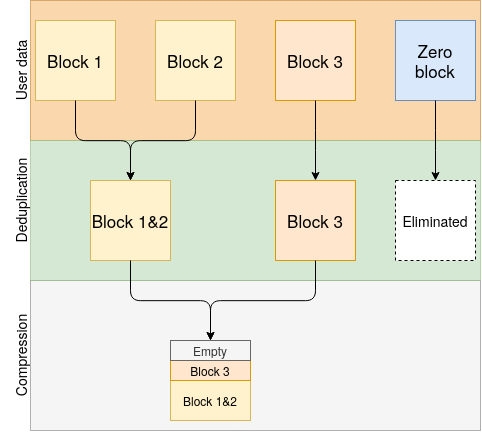
\includegraphics[width=\textwidth]{graphics/diagrams/space_saving.png}
        \caption[Space saving methods in VDO]{Diagram of space saving methods of VDO. In the first step, duplicate data and zero blocks are eliminated. In the second step, remaining unique blocks are compressed and stored as a single block.}
\label{fig:space_saving}
\end{figure}


Deduplication is a technique that, on a block level, dissalows multiple copies of the same data to be written to physical device. In VDO, duplicate blocks are detected but only one copy is physically stored. Subsequent copies then only reference the address of the stored block. Blocks that are deduplicated therefore share one physical address.

Compression is a technique that reduces usage of physical device by identifying and eliminating redundancy in data. In VDO, lossless compression, based on a parallelized packaging algorithm is used to handle many compression operations at once. Compressed blocks are stored in a way that allows the most logical blocks to be stored in one physical block.

The actual VDO technology consists of two kernel modules. First module, called \texttt{kvdo}, loads into the Linux Device Mapper layer to provide a deduplicated, compressed, and thinly provisioned block storage volume. Second module called \texttt{uds} communicates with the Universal Deduplication Service (UDS) index on the volume and analyzes data for duplicates.


\subsection{Deduplication}
Deduplicaton limits writing multiple copies of the same data by detecting duplicate blocks. Blocks that are duplicate of a block that VDO has already seen are stored as references for that block, which saves space on the underlying device.

Deduplication in VDO relies on growing UDS index. Hash from any incomming block, requested to be written, is searched for in the UDS index. In case the index contains an entry with the same hash, $kvdo$ reads the block from physical device and compare it to the requested block byte-by-byte to ensure they are actually identical.

In case they are, block map is updated in a way that the logical block points to the block on underlying device that has been already written. If the index doesn't contain the computed hash or the block-by-block comparison indetifies a difference in the blocks, $kvdo$ updates the block map and stores the requested block.

Either way, the blocks hash is written to the beginning of the index. This index is held in memory to present quick deduplication advice to the VDO volume.

Logical blocks that are copies and therefore share one physical block are called \emph{shared} blocks.

\subsection{Compression}
Another part of VDO optimisation techniques is compression. By compressig already deduplicated blocks, VDO provides one more step to increase utilisation of underlying device. Compression is also importatnt for saving space in case the incoming data are not well deduplicable.

In VDO, lossless compression, based on a parallelized packaging algorithm is used to handle many compression operations at once. Compressed blocks are stored in a way that allows the most logical blocks to be stored in one physical block.


\subsection{Zero-block elimination}
Zero-blocks are blocks that are composed entirely of zeroes. These blocks are handled differently that normal data blocks.

If the VDO layer detects a zero-block, it will treat it as a discard, thus VDO will not send a write request to the undelying layer. Instead, it will mark the block as free on a physical device (if it was not a shared block) and updates it's block map.

Because of this, if user wants to manually free some space, they can store a file filled with binary zeroes and delete.


\section{Constrains and requirements}
VDO layer is in fact another block device that can aggregate physical storage, partitions etc. On creation of VDO volume, management tool also creates volume for UDS index as well as volume to store actual data.

\subsection{Physical Size}
The VDO volume for physically storing date is divided into continuous regions of physical space of constant size. These regions are called $slabs$ and maybe of size of any power of 2 multiple of $\SI{128}{\mega\byte}$  up to $\SI{32}{\giga\byte}$. After creating VDO volume, the slab size cannont be changed. However, a single VDO volume can contain only up to 8096 slabs, so the configured size of slab at VDO volume creation determines its maximum allowed physical size. Since the maximum slab size is $\SI{32}{\giga\byte}$ and maximum number of slabs is 8096, the maximum volume of physical storage usable by VDO is $\SI{256}{\tera\byte}$. Important thing to notice is that at least one slab will be reserved for VDO metadata and wouldn't be used for storing data. Slab size does not affect VDO performance. As mentioned, at least one $slab$ is reserved for VDO metadata and UDS on-disk index.

VDO module keeps two kinds of metadata which differ in the scale of required space.
\begin{compactenum}
\item type scales with physical size and uses about $\SI{1}{\mega\byte}$ per every $\SI{4}{\giga\byte}$ of managed physical storage and also additional $\SI{1}{\mega\byte}$ per $slab$. 
\item type scales with logical size and uses approximately $\SI{1.25}{\mega\byte}$ for every $\SI{1}{\giga\byte}$ of logical storage, rounded up to the nearest slab.
\end{compactenum}

When trying to examine physical size, thee term Physical size stands for overall size of undelying device. Available physical size stands for the portion of physical size, that can actually hold user data. The part that does not hold user data is used for storing VDO metadata.

\subsection{Logical Size}
The concept of VDO offers a way for users to overprovision the underlying volume. At the time of creation of VDO volume, user can specify its logical size, which can be much larger than the size of physical underlying storage. The user should be able to predict the compressibility of future incoming data and set the logical volume accordingly. At maximum, VDO suports up to 254 times the size of physical volume which amounts to maximum logical size of $\SI{4}{\peta\byte}$.

\subsection{Memory}
The VDO module itself requires $\SI{370}{\mega\byte}$ and additional $\SI{268}{\mega\byte}$ per every $\SI{1}{\tera\byte}$ of used physical storage. Users are therefore expected to compute the needed memory volume and act accordingly.

Another module that consumes memory is the UDS index. However, several mechanisms are in place to ensure the memory consumption does not offset the advantages of VDO usage.

There are two parts to UDS memory usage. First is a compact representation in RAM that contains at most one entry per unique block, that is used for deduplication advice. Second is stored on-disk that keeps track of all blocks presented to UDS. The part stored in RAM tracks only most recent blocks and is called \emph{deduplication window}. Despite it being only index of recent data, most datasets with large levels of possible deduplication also show a high degree of temporal locality, according to developers. This allows for having only a fraction of the UDS index in memory, while still mantaining high levels of deduplication. Were not for this fact, memory requirements for UDS index would be so high that it would out-cost the advantages of VDO usage completely.

For better memory usage, UDS's Sparse Indexing feature was introduced to the uds module. This feature further exploits the temporal locality quality by holding only the most revelant index entries in the memory. Using this feature (which is recommended default for VDO) allows for maintaining up to ten times larger deduplication window while maintaining the same memory requirements.

%\subsection{VDO kernel module}
%The $kvdo$ module provides mentioned techniques within Linux device mapper level. Device mapper serves as a framevork for storage and block device management. The $kvdo$ module presents itself as a block device that can be accessed directly as a raw device or via installation of supported file systems (XFS/EXT4). 

%After receiving read request from an above structure, $kvdo$ maps the requested logical address to the actual physical block and retrieves the data.

%When $kvdo$ receives a write reqest, it updates its block map and acknowledges the request. If the received request is either DISCARD, TRIM or a block of only zeroes, $kvdo$ only acllocates a physical block for the request.


\subsection{CPU}
Some of the operations VDO needs to execute in order to effectively save space while remaining highly performing are CPU intensive. These operations such as computing hashes for deduplication or compressing blocks can overload a machine with low computing power

VDO works as a multithreaded application, so it can balance load on multiple cores. Users should regularily check the usage of VDO threads. In case, any thread is using more than 50\% of its CPU, the thread count should be increased to balance the workload better.

\section{Internal supporting structures}
Working VDO instance contains supporting structures that handle the incomming events. Undrestanding their purpose as function is integral to proper performance tuning.


\subsection{Recovery journal}
Recovery journal provides track of all block changes that has yet to be fully, reliably written to the physical device. It provides performance improvement with bothsynchronous and asynchronous writing policies.

When in synchronous mode, the completion request doesn't wait for the change to be made permanent on the device, it merely waits for the ackowledgement from the journal.

In asynchronous mode, the journal helps providing data loss window by ensuring the user will not lose data if the changes are commited to the journal before the window is expired.

The recovery journal has two parts. One is stored on the physical device and the other in memory to serve as a buffer. When entry is added to the journal, it is processed by the part in memory and is regarded as an active block. An attempt to commit the block to the device is made, however, the device might be locked by another commit thats in progress which makes the commit queue. Every successfull commit will wake others waiting after it is completed.


\subsection{Block map}
Block map is a structure used by VDO to handle logical to physical block mapping. It is implemented as a B+ tree and works on a granularity of pages with every page holding mapping of 812 logical blocks.

The full block map is stored on a physical device, in one of the last slabs reserved for metadata and it is a cause of one of the requirements on physical space. It usually consumes about 1.25GB per 1 TB of stored physical data.

Since block mappings are accessed with high frequency and reading from physical device could be costly, part of the block map is stored in memory in a block map cache. When processing incomming request, the relevant page is pulled from the cache, or in case the cache doesn't contain it, it is read from physical device and pushed into the cache. Such cache misses could be costly in terms of performance, and therefore block map cache should be set up coorectly.

\subsection{UDS index}
UDS index is a structure designed specifically to identify duplicate data using hash fingerprints of data blocks. It exists in VDO to provide deduplication advice for effective deduplication. Instance of UDS index is not vital for VDO block handling. In case of losing UDS index, VDO still manages blocks and stores and compress data, only without deduplication. Even in the event of index becoming corrupted, there are different mechanisms in place to assure data correctness, so user can discard the index and start bulding a new one.

Updating index is costly, so VDO is trying to minimise the updates. That is a reason the index can contain references to blocks that are no longer present in data. Those blocks are called stale blocks.


\section{Tunables}
VDO provides user with many means of tuning. Tuning consist of parallelizing workload to more processor by changin number of different threads, choosing the right block map cache size, write policy or discard size.

\subsection{VDO threads}
One of the main means of tuning VDO performance is changing number of VDO threads that are acompleting various tasks. While running a VDO volume, users should monitor the thread usage and tune it accordingly. In case there is a high thread usage (>50\,\%), users should increase the number of relevant threads. There are six tunable threads in VDO. Figure~\ref{fig:VDO-internals} displays relationship between various threads and VDO internal structures.

\subsubsection{Logical zones thread}
Logical space presented to users of VDO device consists of Logical Block Numbers (LBNs).

LBNs are contained within pages, which are the main unit a block map cache is working with. Pages are furhter grouped into zones. Zones are assigned to logical zone threads, such as workload on multiple zones can be managed in paralel

Logical zone threads are active during read and write requests, since they are translating LBNs to PBNs.

\subsubsection{Physical zones thread}
Physical space VDO is working with consists of Physical Block Numbers (PBNs).

PBNs are divided into larger sections called slabs. Every slab is divided into zones. Physical zone threads are processing requests to physical zones in parallel.

Physical zones threads are active only during write phase, because their purpose is to update reference count. vdoPhysicalThreads is the option for seting physical threads.


\subsubsection{I/O submission threads}
I/O submission threads are submiting block I/O (bio) operations from VDO to the underlying physical deivce by passing requests from other VDO threads to the driver of the physical device. 

The number of I/O submission threads can be tuned using vdoBioThreads option.

\subsubsection{CPU and Hash zone threads}
CPU threads and Hash zone threads in VDO help manage and balance intensive computing workload to multiple cores. The intensive operations such as computing hashes or compression are handled by these threads.

The number of CPU and Hash zone threads can be tuned using vdoCpuThreads and vdoHashZoneThreads options respectively.

\subsubsection{I/O acknowledgement threads}
This type of thread is managing acknowledgement operations to an application above VDO after I/O request completion.

The number of ack threads can be tuned using vdoAckThreads option.

%\subsubsection{Journal thread}



\addtolength{\textheight}{1.75in}
\begin{landscape}
\begin{figure}[!hb]
        \centering
        \includegraphics[width=\columnwidth]{graphics/diagrams/vdo_internal.png}
\caption[VDO threads and internal structures]{This diagram displays VDO internal structures and their relationship with VDO threads.}
\label{fig:VDO-internals}
\end{figure}
\end{landscape}
\addtolength{\textheight}{-1.75in}



\subsection{VDO write policies}
VDO can operate in either synchronous or asynchronous mode.\cite{man:writemodes} by default VDO write policy is set to $auto$ which means the the module decides automatically which write policy to use. The main difference is wether or on is the write request written immediately or not. In case of system failure while using asynchronous mode, data can be lost.

\subsubsection{Synchronous mode}
In synchronous mode, VDO temporarily writes the block to the device and acknowledges the request. After completing the acknowledgement, it attempts to deduplciate the block. In case it's a duplicate, block map is updated in a way that the logical block points to the physical block that iss already written and releases the previously written temporary block. In case the block is not a duplicate, $kvdo$ updates the block map to make the temporary physical block permanent.

\begin{figure}[!htb]
        \centering
        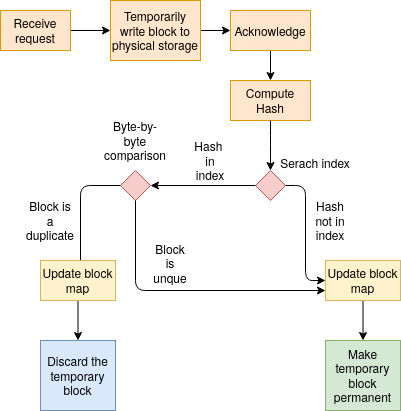
\includegraphics[width=\textwidth]{graphics/diagrams/sync.png}
\caption[Synchronous write mode]{This diagram shows a flowchart of asynchronous diagram processing}
\label{fig:sync}
\end{figure}

\subsubsection{Asynchronous mode}
In asynchronous mode, instead of writing the data immediately, physical block is only allocated and acknowledgement of request is performed. Next, VDO will attempt to deduplicate the block. If the block is a duplicate, the module only updates it's block map and releases the allocated block. If the block is be unique, block map is updated and the data is written to the allocated block.

\begin{figure}[!htb]
        \centering
        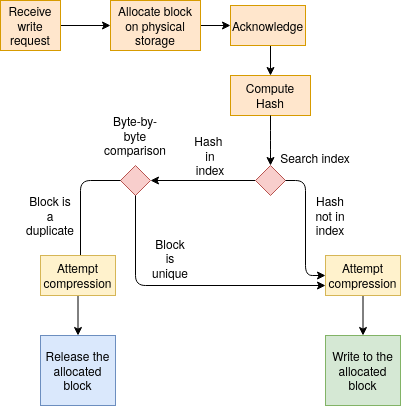
\includegraphics[width=\textwidth]{graphics/diagrams/async.png}
\caption[Asynchronous write mode]{This diagram shows a flowchart of asynchronous diagram processing}
\label{fig:async}
\end{figure}

\subsubsection{Asynchronous unsafe mode}
The option async-unsafe is there in case the user wants to keep the original non-ACID async write policy.


\subsection{Block map cache size}
Block map exists in VDO volume to maintain the mapping of logical blocks to physcial blocks and managed as pages with each page holding 812 entries of logical blocks. The entire block map is kept on disk, since it can be rather large.

Block map cache is a subset of the entire block map that is kept in memory for performance increase. If request to access a block comes to VDO, it will check if that block is in the block map cache. In case it doesn't it needs to read the relevant page and store it in a cache. In case the request was write, it is written in the block map cache and only participates to the on-disk part later.

The block map is a cause of one of the requirements on physical space. It usually consumes about 1.25GB per 1 TB of saved stored physical data. The subset that's kept in memory is much smaller, 128MB by default and is tunable by --vdoBlockMapCacheSize.

The 128MB can cover about 100GB of logical blocks. However if VDO logical space is larger than 100GB and the workload is so random that the requests doesn't hit cached pages, user can observe great preformance hit. In case the block map cache is full, therefore runs out of free pages and a request comes for a page thats not contained in the cache, VDO needs to first discard some page from the cache, write it on disk and just after then load the desired page. It is obvious that this cycle is very time expensive and therefore users are encouraged to increase block map cache size if the precoditions for cache tiering are met.




%\subsection{VDO in Storage Stack}
%\label{stack}
%Generally it is importatnt for users to realise that some of the storage layers work better when above or under the VDO layer in the storage stack.

%Technology that is recommended to be installed under VDO layer:

%\begin{itemize}
%  \item dm-multipath
%  \item dm-crypt, i.e. layer for data encryption
%  \item mdraid, i.e. software raid
%  \item LVM (as software raid)
%\end{itemize}

%Technology that is recommended to be installed above VDO layer:

%\begin{itemize}
%  \item LVM cache, i.e. possibility to mark part of a block device as a cache to be used by LVM
%  \item LVM Snapshots
%  \item LVM Thin Provisioning
%\end{itemize}

%Unsupported configurations are the ones that break those rules plus a few others:

%\begin{itemize}
%  \item VDO on top of VDO volume
%  \item VDO on top of LVM Snapshots
%  \item VDO on top of LVM Cache
%  \item VDO on top of LVM Thin pool
%  \item VDO on top of a loopback device
%  \item VDO under an encrypted device
%  \item Partitions on VDO volume
%  \item RAIDs on top of VDO volume          
%\end{itemize}

%\section{Administering VDO}
%\subsection{Installation}
%Since VDO is now part of Kernel, it can be installed usign native packaging system. VDO relies on two RPM packages to be installed:
%\begin{itemize}
%    \item vdo
%    \item kmod-kvdo
%\end{itemize}
%After succesfull installation of these two packages, user can create a VDO volume.

%\subsection{Creating VDO volume}
%VDO can be created using VDO manager through command line by executing \texttt{vdo create}.
%The required parameters are:
%\begin{itemize}
%    \item --name=vdoname
%    \item --device=blockdevice
%    \item --vdoLogicalSize=logicalsize
%\end{itemize}

%When specifying block device, it is reccommended to use persistent device name. Otherwise, VDO might fail to start properly in case the name of the device changes.

%While specifying the logical space, user should be aware what kind of data will be written into the VDO block device and set the logical size accordingly. If heavily compressible data are expected, user can specify logical size as large as ten times the physical size. If the data are expected to be less compressible, it is reccomended to lower the ratio accordingly.

%After succesfull VDO creation, the layer is prepared to be used as an ordinary block device. That means, either file system can be created on top of it, or a more complex structure can be installed above. All within the contstrains specified in section~\ref{stack}.

%\subsection{Monitoring VDO}
%VDO works as a thinly provisioned volume. Therefore applications or file systems that use it will only see a logical space that is provided by VDO. To monitor VDO space usage, physical space left or compression ratio and much more, $vdostats$ utility provides neccessary inspection of VDO volume.

\chapter{Fs-drift}
\label{fs-drift}

Fs-drift is an open-source benchmark developed specifically for testing heavy workload and aging performance. Being implemented in Python3, it is very easy for users or contributors to add new features or change the benchmark behavior to their needs.

%\subsection{New features}
%Fs-drift was used as a main tool in a previous study of file system aging so only new features will be presented in this thesis.
For performance testing of VDO, new features and behavior needed to be implemented to fs-drift to enable more precise control over IOs and testing process.

\section{Compressible data generator}
While testing compression and deduplication technology as VDO, data generated for testing need to be specificaly shaped. The benchmark needs to be able to generate the testing data in a way that corresponds to examined cases. A restriction for VDO testing is that the repeating patterns in compressible data cannot be composed entirely of zeroes, because the way VDO deals with zero blocks (see, Zero blocks elimination). For this reason, new parameter was added to fs-drift, that enables the user to produce buffers with specified compressibility.

Compressible blocks are achieved by filling the desired number of bytes with random data and filling the rest with zeroes. This way, any generated block is always compressible in desired manner.
%LZ data generator (i.e. lzdatagen) is a simple but powerfull tool for generating data with desired compressibility. The user can specify compression ratio, size and output file and obtains data with those qualities. Seed for repeatable output can be also specified, which is useful for producing deduplicable workload.

%If there is a compression ratio set other than 0.0, the buffer is filled using lzdatagen call with the desired compression ratio. Otherwise the buffers are filled the same way as in previous versions of fs-drift.

%This simple but powerfull feature now empowers the benchmark user to specify the compressibility of written data and therefore makes the user able to measure performance of any technology that deals with compression feature such as ZFS or VDO.

Usage:
\begin{itemize}
    \item -c|--compression-ratio, number that is a desired compress ratio, e.g. 4.0 is a compressibility of 75\%, so the compressed block occupies 25\% of the original space~(default~0.0)
\end{itemize}


\section{Deduplication}
Sometimes it is needed to produce deduplicable data for correct workload shaping. Fs-drift provides this option to users by repeating generated random blocks. Outputed data is therefore deduplicable to a specified amount.

%While some of the data from lzdatagen will be naturally deduplicable, more precise control of deduplicibility of the data could result in more precise performance measuerment.

%As mentioned in the section above, user can input seed value to lzdatagen to produce the same output. Fs-drift uses this parameter to produce deduplicable data. Based on the inputed probability, fs-drift will either produce new data by obtaining new seed from os.urandom() function and saving it for later. In case fs-drift needs to produce data that will deduplicate, it uses one of the stored seed from the previously generated data.

Usage:
\begin{itemize}
    \item -+D|--dedupe-percentage, percentage of data chunks or files that will be deduplicable (default~0)
\end{itemize}


\section{DirectIO}
When researching behavior of random operations in fs-drift, file system cache can often skew considerable amount od measurements.

%This could affect reads, since the blocks could be read from the cache instead of the device.

The system cache considereably affects both writes and reads, and the effect is mostly visible with random operations. In fs-drift, $fsync$ time was taken into the measurement to get the real request completion time. However, the system cache succesfully serialises the requests, so at the time of fsync, they are written sequentially.

To battle this effect, option to use direct IO was added. When passing os.O\_DIRECT flag to the os.open() call, the UNIX based systems require memory alignemnt to the underlying device so all the operations had to be refactored into being aligned.

Usage:
\begin{itemize}
    \item -D|--direct, if 1, use os.O\_DIRECT flag when opening files. Data alignment of 4096 bytes will be used. (default 0)
\end{itemize}

\section{Rawdevice}
While file system can be installed on a VDO layer (and there is an increasing number of users which do), it is important to have an option to test VDO block device also without the file system to get more precise measueremts. File systems can have considerable impact on performance and can skew results in ways that make it hard to clearly observe VDO impact on overall performance.

Rawdevice mode was added, that enables fs-drift to run block-wise on a given device instead of working with files on a file system.

Usage:
\begin{itemize}
    \item -R|--rawdevice, set path of the device to use it for rawdevice testing (default '')
\end{itemize}


\section{Random discard operation}
With thinly provisioned technology being increasingly relevant, it is interesting for researchers to also test performance of a block discards. Discard command could be passed either from the file system or an application to let the underlying device know that the particular block is no longer occupied and can be returned to the block pool.

In Linux, available command for block discard is $blkdiscard$. User can specify the offset and length to be discarded, making it very easy to write an operation type for fs-drift.

The pilot idea was to call blkdiscard command using the subprocess module. However, discard operations are very fast and the speed of calling subprocess module has become a significant bottleneck.

Howver, Python provides a framework to execute ioctl calls directly from the Python code. First, the code for BLKDISCARD operation needs to be computed. Parameter for BLKDISCARD ioctl is an array of two u\_int64 numbers which represent the beginning offset and length to discard. This structure can be created by using Pythons module $struct$. Example~\ref{ex:blkdiscard} shows exactly how to issue block discard ioctl.

If the users of fs-drift wants to test discard speed, they can specify so in the configuration file along with a probability of the event. When the event of discard is triggered, fs-drift works similar as with random writes, but intead of producing buffer and writing data, it's using discards with random offset and specified block size to call BLKDISCARD.


\lstset{language=Python, 
numbers=none, 
frame=single, 
commentstyle=\color{blue}, 
basicstyle={\scriptsize\ttfamily}, 
keywordstyle=\color{blue}, 
%identifierstyle=\color{blue}, 
stringstyle=\color{red},
captionpos=t,
showstringspaces=false,
breaklines=true,
breakatwhitespace=false,
tabsize=3,
caption={sdad},
}


\begin{lstlisting}[language=Python, caption={Using BLKDISCARD ioctl to discard first 4096 bytes of a device /dev/sde},label={ex:blkdiscard}][frame=single]
import os
import struct
from fnctl import ioctl
offset = 0
length = 4096

#opening a device that supports BLKDISCARD
fd = os.open('/dev/sde', os.O_WRONLY)    

#computing command for ioctl,
#the value from documentation is _IO(12, 119)
BLKDISCARD =  0x12 << (4*2) | 119

#Creating C-like array of two uint_64 numbers
args = struct.pack('QQ', offset, length)

#Finally, ioctl call with the prepared parameters
ioctl(fd, BLKDISCARD, args, 0)

os.close(fd)
\end{lstlisting}


\section{Random map}
When computing offset for random operations, it might not enough to just generate random number. Sometimes it is benefical to administer IOs only to unused blocks, ensuring no overwriting takes place and all the free blocks will eventually be used.

For this purposes a feature to keep track of unused offests was added to fs-drift. The random map is generated before the test as a shuffled list of possible indices, to save time while the workload is in progress.

The user should be wary of the fact that if the test runs out of the random map, it is recomputed again and will start to overwrite data.

Usage:
\begin{itemize}
    \item -r|--randommap, if true, use random map to get random offsets (default False)
\end{itemize}

\section{Multithread}
Multithreaded workloads are essential for researching performance of ------.

Option to run fs-drift a multithreaded bechmark was added. User will just specify the number of threads that is to be used and fs-drift will spawn that many. For this option, large parts of fs-drift needed to be reengineered so the threads are not corrupting eachother data structures, buffers, etc.

Important fact to notice is that every thread is maintaining its own performance throughput report so it is expected that the user will know how to aggregate and interpret the result.

If multithreaded fs-drift is used for testing, user should limit the number of parallel IOs using iodepth parameter.


\begin{itemize}
    \item -T|--threads, fs-drift will spawn this many threads to run a workload (default False)
\end{itemize}

\section{IOdepth}
Fs-drift threads will submit their IO requests to the device or files in parallel. By default, this behavior is unmanaged and can result in overloading or starving the target.

By using iodepth parameter, user can specify how many 4k IO units will be submitted at the same time. This behavior is implemented by managing a counter shared between threads. This counter contains information on how many IOs are in progress. If this number is higher or the same as the specified iodepth, threads will wait for the counter to be lowered. If a thread is in its preparation phase and the IO depth is full, it will compute larger buffer of random data, so the workload is more effective.


\begin{itemize}
    \item -i|--iodepth, number of 4k blocks that can be executed at the same time (default 0)
\end{itemize}



\section{Performance measurement}
In fs-drift, performance is measured by saving a time stamp before invoking the IO operation and storing the time stamp difference after the operation was finished. However, with this type of measurment, it is important to make sure the time stamping is as close to the actual IO operations as possible. 

In previous versions, the time measurement was the same for every IO operation, which made some of the measurement incosistent, e.g. taking into the measurement the time to generate buffers, setting offset to file descriptors. etc.

This problem was removed by moving the time stamps inside the functions, providing more precise control over the timing of events.

Another small feature added by switching to $perf\_counter()$ as a tool to log time instead of $time()$.


\section{Data reporting}
In previous versions, data was stored in the programs memory which increased RAM consumption during long tests. Also in case of OS or benchmark failure all the results were lost. This problem was removed by having the output files open and continually appending new entries.

In fs-drift, gathering only response (completion) times introduced noise to the datapoints, since there can be variability of file or data size, that variability will directly project into the data, since working with larger files can take longer than working with smaller files.

With this in mind, an option to store bandwidth was added as a new feature. Bandwidth is measuerd as a total completed size divided by the time of completion. This way, variability of data size is not affecting the measurements.

%\section{FIO}
%Flexible Input/Output tester is a workload generator known for its flexibility and large base of users and contributors. It is an exellent benchmark for testing block devices and file systems since it gives users very precise control over the workload.

%\subsection{for testing VDO}


\chapter{Testing methodology}
\label{methodology}
This chapter presents used testing hardware, setup of testing environment and performance measuring methodology.


\section{Testing environment}
While testing performance, usage of clean testing environment is strongly encouraged. In time of testing, no other applications should run in the environment to ensure low noise levels. Running tests on clean installation of OS is prefered to ensure no performance impacts caused OS aging, memory shortage, etc.

For this thesis, testing was conducted on instances of RHEL-8.1 and RHEL-8.2 to gain access to the most recent features. Tuning options for the systems were set to $throughput-performance$. Other options for the OS are left to be default.

Storage stack for testing purposes is always prepared by executing a seuqence of LVM commands. For the simples tests, one volume group and one logical volume was used to be a block device for VDO layer.

The storage stack can be tested either as a raw deveice, or file system can be installed on top of it when working with files, or relationship between stack and file system needs to be examined.

It is important to create a fresh instance of stack before the test to ensure stable testing conditions. Also, before every test, we $sync$ and $drop caches$. 

\subsection{VDO allocation}
\label{alloc}
Reproducibility of results is an important aspect of any kind of testing. As mentioned, new test environment is prepared before every test to achieve stable, reproducible results. However, when VDO instance just started, it's mapping information is not fully allocated yet. VDO stores its mapping information in a tree, which is allocated as needed.

This could pose a problem for performance testing, since the allocation takes some to complete and therefore some amount of testing time will be testing the allocation latency. We can observe this effect on a Figure~\ref{fig:emptyVDO}. This test was conducted on a empty instance of VDO on top of HDD device. As could be observed, it took about 150s for VDO to reach stable performance.

In case we don't want to specifically test VDO allocation latency, by testing on unallocated VDO a large of testing time is effectively wasted. This could be avoided by forcing VDO to allocate all of its mapping tree before the test. VDO logical space is divided into regions of 812 4k blocks. Every region is covered by the same set of mapping blocks. Therefore executing a write request to each region will force VDO to allocate the whole needed mapping tree. 

We can achieve the allocation f.e. by writing zero byte every 812*4096 bytes through all the logical space before test. Figure~\ref{fig:preallocatedVDO} shows performance of VDO measured after executing the preallocatig sequence. We can observe, that the performance is stabilised from the start of the test unlinke the previous test.

This technique will be by default used prior to all further tests, unless explicitly stated otherwise. The operation is a component of the testing package and can be controlled by parameter -a.

\clearpage
\begin{figure}[!h]
        \centering
        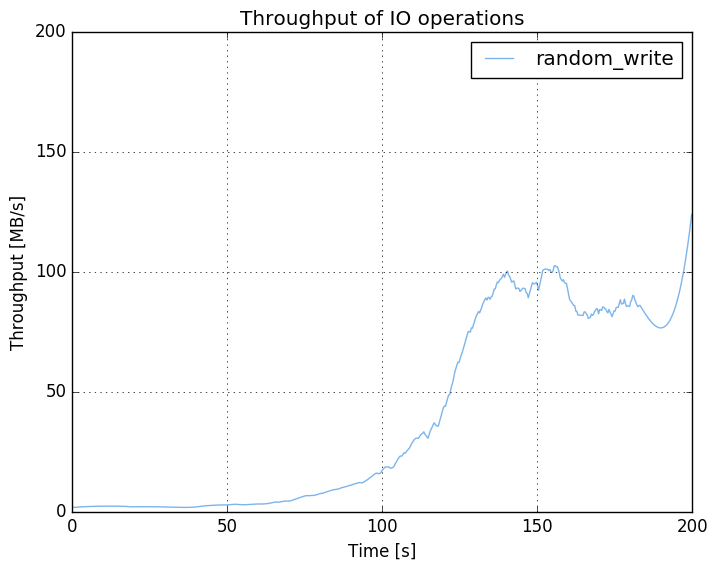
\includegraphics[width=\textwidth]{../results/empty_VDO/HDD/tar_467_bw}
\caption[Performance of unallocated VDO storage]{Performance of allocated VDO storage in time. After all mapping space is allocated, the performance stabilises.}
\label{fig:emptyVDO}
        \centering
        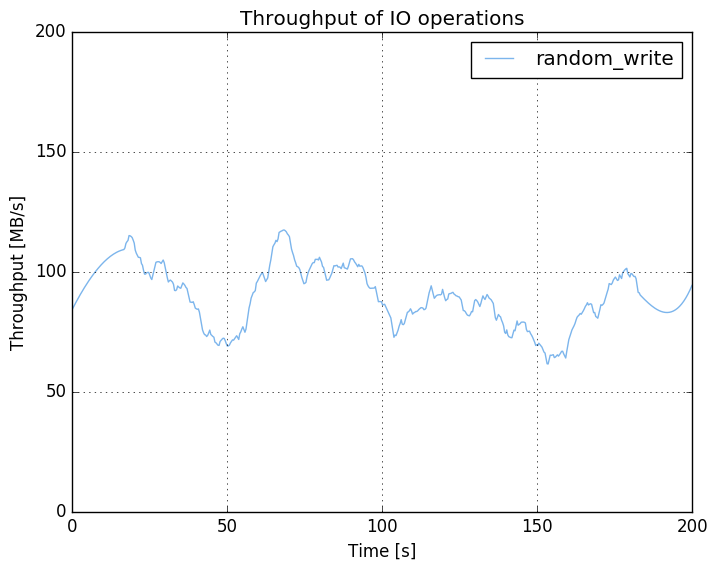
\includegraphics[width=\textwidth]{../results/empty_VDO/HDD/tar_224_bw}
\caption[Performance of allocated VDO storage]{Performance of empty, but previously allocated VDO storage. Measurements are stable through the whole test.}
\label{fig:preallocatedVDO}
\end{figure}

\clearpage


\section{Testing with fs-drift}
Fs-drift is a powerfull tool for administering IOs, simulating many types of workload. To obtain correct performance measurements, it's important to setup benchmark correctly.

\subsection{File size}
File size is another parameter that need to be carefully thought of. File size is used both for testing on file system and testing with rawdevice. It represents the size of data that will be administered block by block to the device or file. Again, since there is some delay between actually invoking the writing process, larger file size will mean more aggresive workload for the device or file system. It is also a granularity at which fs-drift collect data, one record for a given file, so seting file size too high can mean lowering the data points in results.

\subsection{Block size}
Choosing the correct block size for the workload is a very important step. For most cases, the native VDO blocksize of 4k is used. However, it is important to understand what does choosing different blocksize mean for the workload.

The way fs-drift works, block size is the smallest granularity of IOs that will the workload achieve, which means that it is a smallest chunk of data that will be submitted to the device or file. Since there is some work to be done between the subsequent submisions, the device that services the requests can have a small bit of time to process the requests. By choosing larger blocksize the workload becomes more aggressive, since there is more data submited at the same time.

However, by increasing block size, we're increasing the smallest continuous chunk of data that will be worked with, so a random workload may become slightly more sequential.

\subsection{Compression ratio}
Compression ratio is a very imporant factor while testing VDO. Generally, it is good to use some compression, so the VDO can excercise all its components. However there can be cases where lowering the compression ratio would benefit the user, f.e. if the goal of a test run is to fill as much of physical space as possible, it would be counter-productive to let a portion of the data be deduplicated and compressed.

While testing VDO, it is important to remember that it's using packaging compression and storing compressed fragments in one block. In case the compression ratio of written blocks is lower than 50\%, therefore resulting compressed blocks would occupy more than 50\% of their original size, there will be no apparent compression during the test, because the packaging algorithm would not be able to fit multiple blocks into one.

\subsection{Deduplication}
Similar to compression, it is expected that user data will be to some degree deduplicable and the testing workload should reflect that. Fs-drift is producing deduplicabla data on a file-size granularity.

\subsection{Random map}
Most testing workloads that aim to test limits of VDO technology are random writes. This also excercises the ability of VDO to serialise workload for the device underneath. By default, fs-drift is randomly choosing the offset to write the next block of data.

However, this approach may not be best, since some blocks can be used more than once and some blocks may never be used. The act of overwriting blocks can introduce noise to the results, so in case the test is not specifically aimed at reusing blocks, it is reccomended to use randommap.

\subsection{Multithread and maximal performance}
VDO is a high performing layer aimed to serve intensive, multithreaded applications. As a block device, VDO serves incoming IO stream through a queue of 2000 IOs. In the test aimed to excercise upper limits of VDO performance, the generated workloads need to be intensive enough so the full potential of VDO can be achieved.

To generate such workload, we need to use multithreaded fs-drift with batch submition controled by iodepth. Iodepth in fs-drift controls exactly how many 4k blocks will be in progress at any given time. It is not only lower, but also upper limit of the batch size.

By setting these parameters correctly, we aim at the right VDO queue excercies. If the VDO isn't engaged enough, the test is limiting itself in the performance. On the other hand, if the test has no upper limit on IO submission, the queue would be overflown at all times, which will slow down performance.

Following formula references a way to compute maximal batch size with given number of threads and block size.

\[ threads * (blocksize \ 4) = Maximal batch size \]

In case the maximal batch size of the test with given parameters is much larger than 2000 (size of VDO queue), the test will overwhelm VDO and measued performance would be too low. In case the maximal batch size of a test is much smaller than 2000, the test will not excercise VDO fully and the performance would also appear low.

Fs-drift parameter iodepth limits the batch size from both size. If the user specifies iodepth of 2000, fs-drift will be submitting exactly 2000 4k blocks at the same time.

However, even limiting batch size with iodepth isn't a final solution. In case the physical device under VDO is very slow, VDO might not be able to empty the queue between batches which would again cause delays and worse performance. Testers should always make sure the queue was properly excercised by inspecting vdostats during and after the tests.

\section{Testing package}
To manage the test results and metadata as well as testing environment and to be able to include tests in more complex or automised workflows, it is beneficial to encapsulate the benchmark into a testing package. For fs-drift, there is drift\_job package.

Drift\_job accepts several parameters such as used device, command for preallocation or parameters for fs-drift. When run, it prepares the testing environment, gathers data about the system, runs the test and package results into an easily managable tar file. The results can be then automatically sent to a data gathering server.

If specified, the package also asynchronously gathers information while the test is running such as statistics about VDO volume. However, since starting phase of fs-drift may take considerable amount of time (allocation, computing random map), the gathering thread waits for fs-drift start file. This functionality is used mainly to gather statistics about VDO using vdostats, however other points of interest may be stored for later examination using this feature.

%While fs-drift doesn't run on itself as a multithreaded program, there is a small support hidden away as prefix parameter. This prefix, when used, will be used as a prefix to object that particular instance of fs-drift works with.

%This makes it possible to actually run multithreaded tests using this testing package. Drift\_job takes a parameter THREADNUM and the it runs that many instances of fs-drift as concurent threads. All the results are stored in a single package, but as multiple files, so then they might be examined in different ways.

\section{Data processing}
Data processing is accomplished by using library written for processing drift\_job packages. The main object Report will process data from all the specified result packages and creates easy to view html report.

The html report consists of two parts. First part is presenting individual report for given results. The second part is comparing the inputed results in an easily digestable manner.

The report output can be tuned with several parameters:

\begin{itemize}
    \item list of paths to individual tar packages
    \item path to store the output
    \item offset, tuple to control which part of X axis to view
    \item log window, for approximating data points
    \item smooth, to let the object know if interpolation and filtering should be used
    \item chart\_vdostats, list of vdostats atributes to plot
    \item lim\_Y to set the upper limit of Y axis
    \item test\_label, to label outputed comparing charts
\end{itemize}

%Data processing script is working exclusively with the files generated by the testing package drift\_job. It will open the package and create its own data objects producing a report.

%The report contains metadata gathered by the test as well as many different charts and statistics.

%The data processing scripts accepts many parameters so we can compare different test runs and tune the output.


\subsection{VDO chart}
In case the test was run on a VDO volume, the resulting tarball will contain a file with vdostats logs. The data processing script will find all the statistics the user inputs and produces a chart. This chart therefore shows the state of VDO in time, while the test was running. We use it mainly to view how many logical and physical blocks were used. But with testing specific components like block map cache or journal, we can view their statistics easlily on this chart

\subsection{Throughput progression chart}
This chart is a simple representation of a measued throughput during the test. Since the data can be sometimes noisy, filtering and interpolation is used to obtain a smooth curve. The way filtering with Savitzky-Golay filter works, if there are revolting data points on the extremes of the X axis, it will cause the curve to turn up or down in hyperbolical maners. If this happens and it hinders the visibility of the results, offset can be set accordingly so the revolting values are excluded.

This chart is mainly used to confirm there was no event that would speed up or slow down the test. If there is a dramatic change in a throughput progression that was unexpected, the test might be faulty.

Hower, it is very usefull, when there is an expected change in behavior of the underlying device such as Empty VDO or Half-Full VDO test

\subsection{Histograms}
%Histogram of measured throughput is an excellent tool to observe some effects when testing. On this chart, we can usually observe if there are different structures servicing IOs during our workload such as cache.

\subsection{Boxplots}
Boxplots are the main tool used to visually compare performance of different tests. The part in focus is the median, which is the main metrics considered when comparing multiple test runs.

\section{Testing hardware}
Testing for this thesis was conducted on multiple machines provided by Red Hat company. I will introduce testing systems which will be used for multitude of tests with or without the VDO layer installed. These machines were chosen by their computing power, provided memory and by useful storage hardware they are equiped with. These machines are stable systems used by Red Hat Kernel Performance team for regular testing.



\chapter{Performance of VDO}
\label{testing}


\section{VDO aging}
\label{half}
VDO will try to serialise the the incomming workload if possible by sequentially filling slabs to about half of their capacity. If more than half of slab is used, or if VDO is running out of free physical blocks, it will start to search for free blocks in the slab, which will appear as a change in performance. 

When VDO is empty, the performance can look as of preformance of underlying device under sequential load. After using about 50\% of the physical capacity, performance will lower and starts to resemble a performance of underlying device under random workload. Figures~\ref{fig:half-start} and Figure~\ref{fig:half-end} show change of access pattern of VDO to an underlying device.

We could test this effect by setting up fresh VDO volume, preallocating it and running random write workload without randommap. This means some of the blocks might be overwritten during the workload, which can free some physical blocks from the sequentially filled slab, that the VDO can search for.

While running this test, performance of VDO should be reasonably stable until it uses about half of its data blocks. Performance should sharply decrease after that point.

On Figure and Figure, results from such test can be examined. Physical space for this test was set to 5g with slab size of 2g, therefore this instance of VDO has one slab of data blocks. We can observe on the Figure that the workload caused the VDO to use half of its datablocks in about 120s. While looking at the Throughput graph, we can see that is the turing point for performance decrease.


\begin{figure}[!htb]
        \centering
        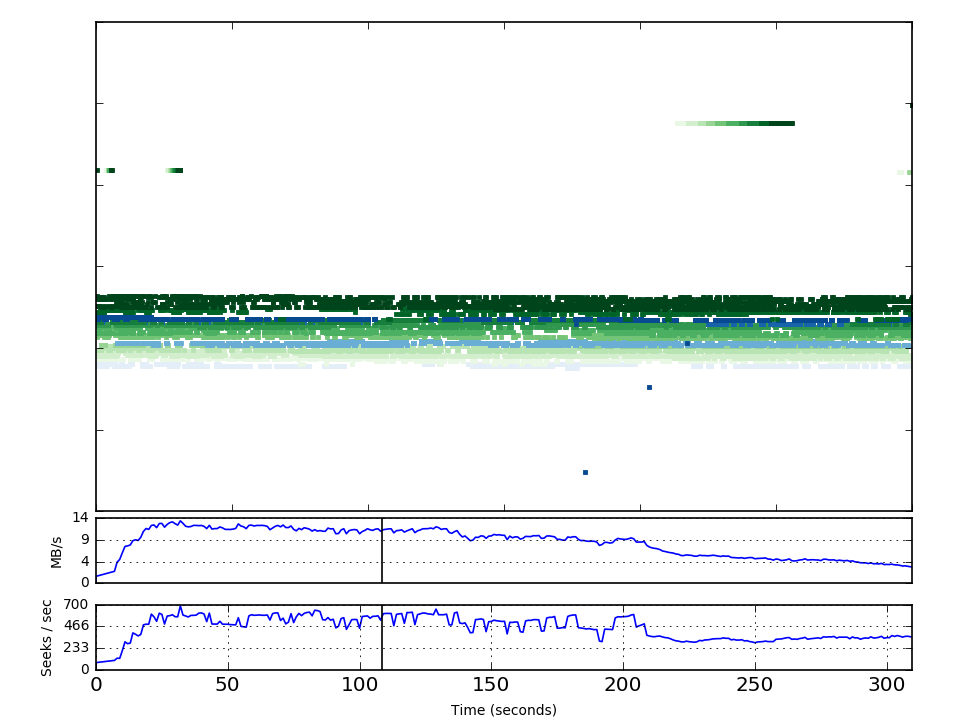
\includegraphics[width=\textwidth]{../results/half/start}
\caption[Access pattern of VDO with enough free space]{Access pattern of VDO to the underlying device while VDO is empty. VDO is successfully serialising incomming workload.}
\label{fig:half-start}
        \centering
        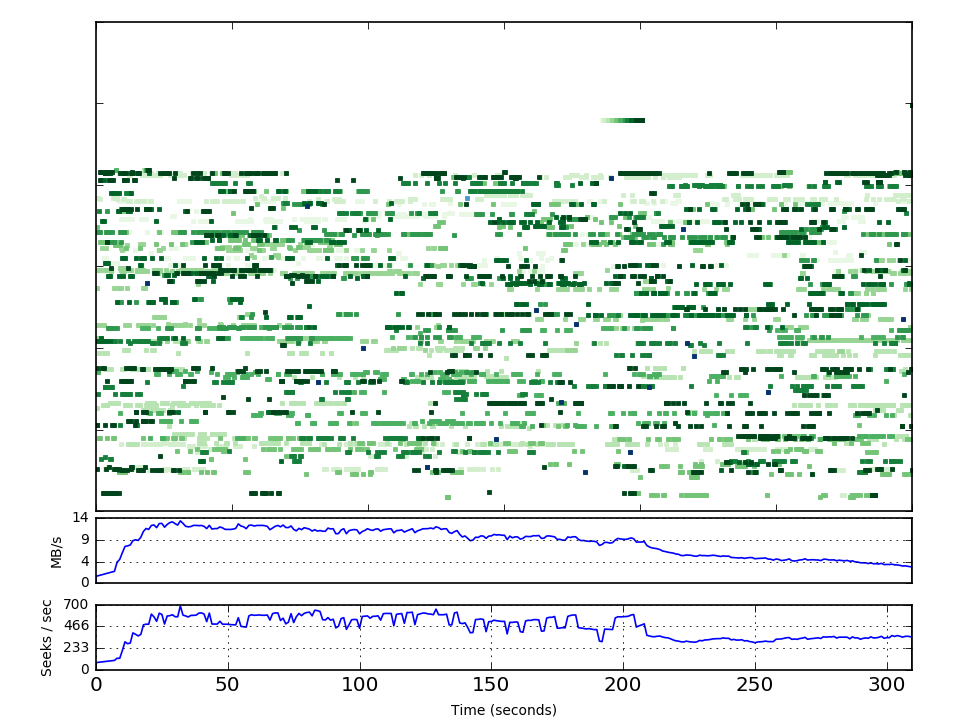
\includegraphics[width=\textwidth]{../results/half/end}
\caption[Access pattern of VDO running out of free space]{Access pattern of VDO to the underlying device while VDO is almost full. VDO can't serialise incomming workload anymore.}
\label{fig:half-end}
\end{figure}


\section{Steady state testing}
As shown in Sections~\ref{half} and ~\ref{alloc} performance testing of VDO is suspectible to various testing preconditions. Most of the VDO instances created by users won't be unallocated nor will they be only half empty most of the time. To find out, how could VDO perform while being used in real-life, we should be able to create a testing instance that would show qualities of used VDO.

The aim of this test is to bring VDO to a hypothetical steady state where its partially fragmented and almost full. This can be done by dividing the testing to two stages. First stage will be aimed to prepare the VDO volume. Second stage will finally gather performance measurements.

The prewriting should fullfill these conditions:
\begin{itemize}
    \item fill up more than half of physical space
    \item use random write accross the logical space so the content is cached
    \item no compression and deduplication
\end{itemize}

\clearpage
\section{VDO threads}
Setting the correct number of VDO threads is the main method for users to increase performance. Incorrect amout of threads can result in unwanted performance penalty.

To show the effect of VDO threads tuning, we'll design a workload that could exercise VDO in a way it will benefit from thread count increase. The designed workload will mimic high-trafic, multithreaded usage. We'll use high thread count, large block size, random write workload without randommap, so the data can be randomly overwritten. To generate more traffic, occassional large discard will be triggered so the physical space becomes more fragmented.

We can see results from VDO threads testing below. The tests were conducted on Machine~\ref{hw:2} with VDO installed on an SSD. Each test, number of threads was increased to show the optimal performance. The conducted tests were:

The prewriting should fullfill these conditions:
\begin{itemize}
    \item default: Logical: 1, Physical: 1, CPU: 2, Hash: 1, Ack: 1, Bio: 4
    \item 1: Logical: 1, Physical: 1, CPU: 1, Hash: 1, Ack: 1, Bio: 1
    \item 2: Logical: 2, Physical: 2, CPU: 2, Hash: 2, Ack: 2, Bio: 4
    \item 3: Logical: 4, Physical: 3, CPU: 3, Hash: 3, Ack: 4, Bio: 6
    \item 4: Logical: 6, Physical: 3, CPU: 4, Hash: 3, Ack: 6, Bio: 8
    \item 5: Logical: 8, Physical: 6, CPU: 6, Hash: 3, Ack: 6, Bio: 8
\end{itemize}

On Figure~\ref{fig:CPUdefault} it is apparent that the thread count is insufficient. Not only does the one Logical thread use up to 80\% of CPU, usage of some other threads is nearing 40\%. This is mainly Physical threads and CPU and Hash threads (The complete results can be found in electronic appendix).

Figure~\ref{fig:CPUtuning} it is observable the CPU usage of individual threads was lowered after increasing the threads number. We can examine the performance impact in Figure~\ref{fig:threads-all}.

By examining the exact values in Table~\ref{tab:tuning}, we can see that the correct thread tuning improved throughput by approximately $\SI{100}{MBps}$.

\begin{figure}[!htb]
\begin{minipage}{.5\textwidth}
        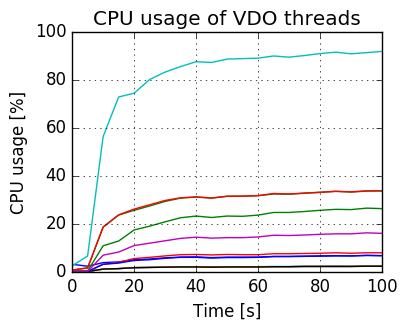
\includegraphics[width=\linewidth]{../results/threads/direct/low_res/tar_695_threads.png}
\caption[VDO threads load on default setting]{Thread load before increasing number of threads (Test: default)}
\label{fig:CPUdefault}
\end{minipage}
\begin{minipage}{.5\textwidth}
        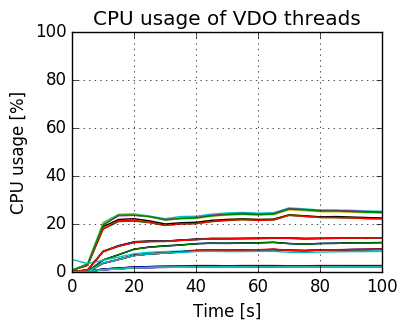
\includegraphics[width=\linewidth]{../results/threads/direct/low_res/tar_770_threads.png}
\caption[VDO threads load after tuning]{Thread load after increasing number of threads (Test: 5)}
\label{fig:CPUtuning}

\end{minipage}
\end{figure}

\begin{figure}[!htb]
        \centering
        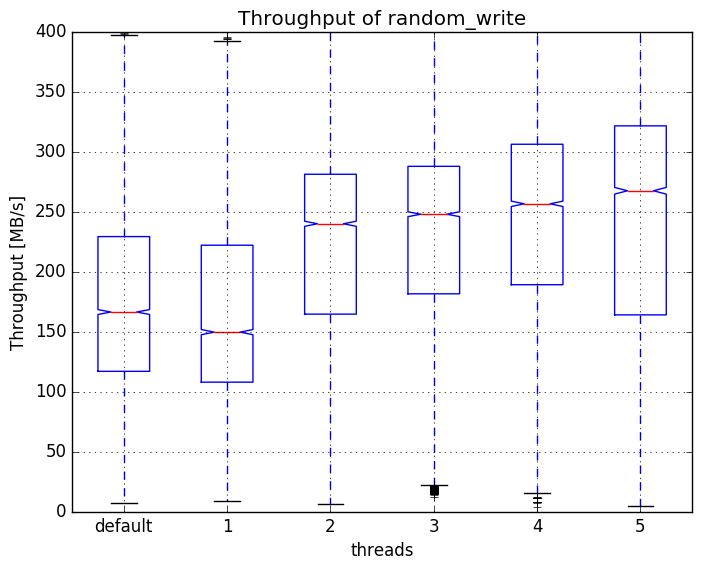
\includegraphics[width=\textwidth]{../results/threads/direct/low_res/random_write1_compare_boxplots}
\caption[Tuning performance by increasing number of VDO threads]{Testing of VDO volume created with increasing numbers of VDO threads}
\label{fig:threads-all}
\end{figure}

\begin{table}
\begin{tabular}{|l|l|l|l|l|l|l|}
        \hline
        \multicolumn{7}{|l|}{Throughput of random write (MB/s)} \\ \hline
        & median & 1st q. & 3rd q. & min & max & stdev \\ \hline 
default & 166.24 & 116.82 & 229.1 & 6.99 & 953.87 & 89 \\ \hline
1 & 149.48 & 107.79 & 221.91 & 9.08 & 1130.06 & 94 \\ \hline
2 & 239.78 & 164.48 & 281.05 & 6.48 & 1241.21 & 125 \\ \hline
3 & 247.74 & 181.42 & 287.65 & 11.74 & 1366.39 & 125 \\ \hline
4 & 256.41 & 189.02 & 306.05 & 4.12 & 1664.54 & 141 \\ \hline
5 & 267.29 & 163.87 & 321.38 & 4.89 & 1400.84 & 153 \\ \hline
\end{tabular}
\caption[Tuning performance by increasing number of VDO threads]{Results of performance tests of multiple tests with increasing number of load balancing VDO threads}
\label{tab:tuning}
\end{table}

\section{Block map cache}
%As mentioned in Chapter~\ref{vdo}, block map cache is an internal VDO structure that keeps part of the journal in memory to provide better performance. Its default size is 

When VDO receives a request, it needs to find mapping between the logical and physical address in the block map. First, it looks for the needed entry in the pages stored in block map cache. If it's not in the cache, VDO will retrieve the correct page from the part of block map that is stored on the disk and writes the page into the block map cache. If the request was a write request, page is updated only in memory and the change will be written to the on-disk part when VDO decides to discard the page from the cache.

VDO decides to discard pages from the cache either when it wasn't used for some time of if there is no space for a new page to be cached. If there is no space left in the cache, VDO needs to discard some page, writing it on the device and load the requested page. This round trip of two I/Os to the physical device is expensive and could cause a performance problem.

The default size of block map cache is $\SI{128}{\mega\byte}$, which is XXX pages, that covers about $\SI{100}{\giga\byte}$ worth of data. In case the logical space is larger than what could be managed by the block map cache and the access pattern of the workload is unpredictable enough, block map cache can easily run out of free pages and would need to write and load a page to and from the physical device on every request. That could be a bottleneck for VDO performance and is the reason why users can increase the size of a block map if they believe the standard size will not suffice.

To test this effect, an unpredictable, aggresive random write workload can be run on VDO instances with various sizes and various block map cache sizes.

The test results show performance of random write workload on three VDO instances. Al the parameters of VDO were kept the same except logical size, and block map cache size:
%In case the logical space is large enough and the workload access pattern causes the cache to fill up completely in a way the block map cache is tired out. If the block map cache fills up, (runs out of free pages), and there is a write request to a non-cached page, the cache is forced to discard one page from its pool to make room for the relevant page. This operation is very costly and this could become a bottleneck for VDO performance.


%If the block map cache runs out of free pages, it is forced to discard one page and load the need one (which is written to) from disk. This operation is very costly and this could become a bottleneck for VDO performance.

%To test this effect, we can use random, unpredictable write workload on an instance of VDO with sufficient and insufficient cache size. The parameter to tune cache size in VDO is --blockMapCacheSize=BYTES.

%To ensure the workload is truly aggresive, parameter randommap and large file size is used so the test makes lots of requests in a short amount of time and there is no chance that the requested blocks will be in the cache.

%To ensure the workload is truly aggresive, large file size and completely random write is used so the test makes lots of requests in a short amount of time and the effect of caching pages could be seen.

\begin{itemize}
    \item Test1: logical size: 80g, block map cache size: $\SI{128}{\mega\byte}$(default)
    \item Test2: logical size: 400g, block map cache size: $\SI{128}{\mega\byte}$(default)
    \item Test3: logical size: 400g, block map cache size: $\SI{512}{\mega\byte}$ 
\end{itemize}

The expected results will be that on the VDO volume with insufficient cache size, performance will be singificantly worse than on other two tests. The test with increased cache size will demonstrate, that the standard performance is restored to the baseline levels.

We can observe the comparison of performance on Figure~\ref{fig:blockmap-boxplots} and Table~\ref{tab:blockmap-tab} for exact numbers.

\begin{figure}
        \centering
        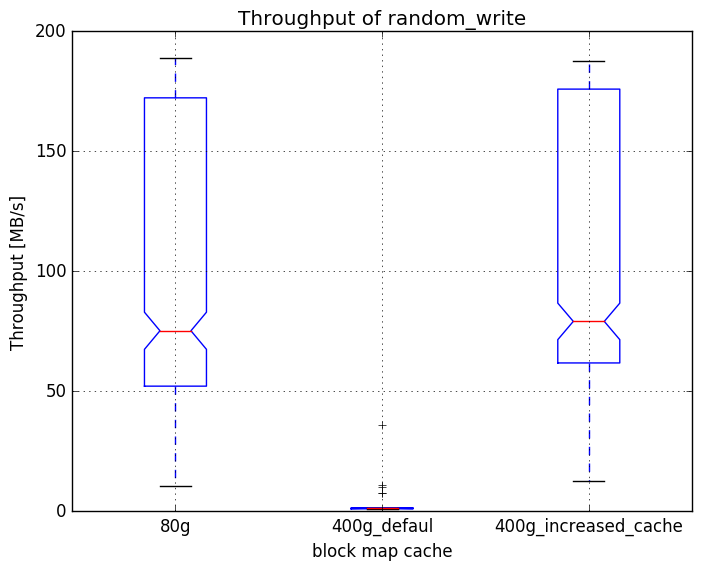
\includegraphics[width=\textwidth]{../results/block_map_cache/report/random_write1_compare_boxplots}
\caption[Block map cache size testing]{Testing of VDO volume created with sufficient and insufficient block map cache size}
\label{fig:blockmap-boxplots}
\end{figure}

\begin{table}
\centering
\begin{tabular}{|l|l|l|l|l|l|l|}
        \hline
        \multicolumn{7}{|l|}{Throughput of random write (MB/s)} \\ \hline
        test name & median & 1th q. & 3rd q. & min & max & stdev \\ \hline 
80g & 67.32 & 46.16 & 151.54 & 10.57 & 188.82 & 55 \\ \hline
400g defaul & 1.13 & 0.94 & 1.32 & 0.85 & 35.98 & 1 \\ \hline
400g increased cache & 74.66 & 58.18 & 174.05 & 12.69 & 187.58 & 55 \\ \hline
\end{tabular}
\caption{Testing of VDO volume created with various with sufficient and insufficient block map}
\label{tab:blockmap-tab}
\end{table}



\section{Maximum discard size}
Performance of discard operation is important to consider, since users may want to discard large quantities of blocks to free space.

VDO offers an option to change the maximum allowed discard size with a parameter --maxDiscardSize. VDO will process discards one VDO block at the time to ensure metadata consintency. VDO manual states that lower discard sizes could work better since, VDO can process them in parallel, assuming low IO traffic.

The tests of maximum discard size throughput were conducted on four different VDO volumes created with differend --maxDiscardSize parameter. This progression was tested on empty VDO, full VDO and empty VDO with preallocation.

The results from unallocated empty VDO are not considered, since it is not expected for users to work (and perform discards) on unallocated space.

While processing the data, the interesting statistic to look for from vdostats is \texttt{bios in discard}. By observing bios in discard together with logical blocks used and with the progession of throughput, we can see the relationship between performance of discarding data and performance of discarding empty blocks.


\begin{figure}[!htb]
        \centering
        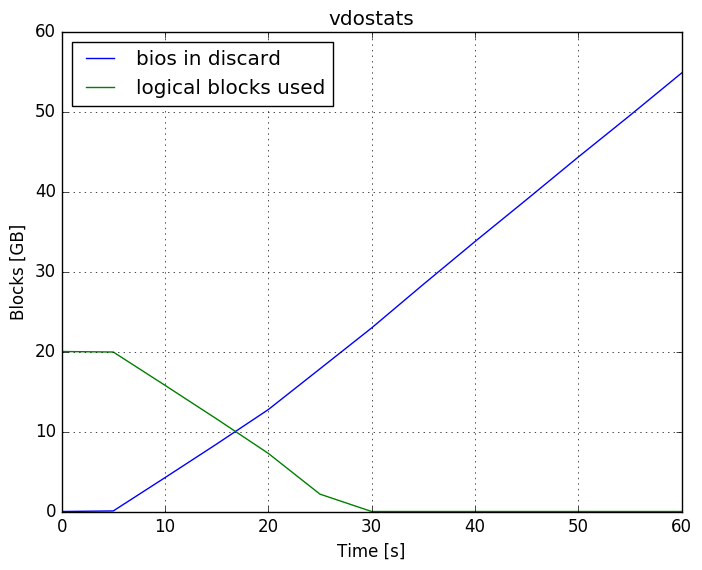
\includegraphics[width=\textwidth]{../results/discards/full_VDO/report/tar_184_vdostats}
\caption[Evolution of VDO stats during random discard workload]{Evolution of VDO stats during random discard workload}
\label{fig:discard-full-vdostats}
        \centering
        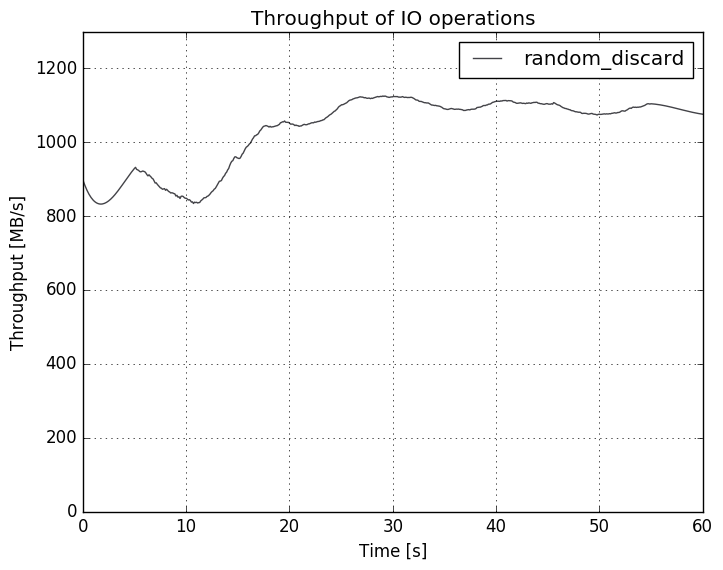
\includegraphics[width=\textwidth]{../results/discards/full_VDO/report/tar_184_bw.png}
\caption[Evolution of throughput during random discard workload]{Evolution of throughput during random discard workload}
\label{fig:discard-full-througput}
\end{figure}

As we can see on the Figure~\ref{discard}, while having normal VDO setup and regular discard workload, the speed of discard operation is decreasing with using larger discard sizes. This test was conducted after a previous run of fs-drift filled all the space with random writes. Filling the storage with random data before every test takes a considerably long time. To shorten the time to test discard operation, we could try testing without prewriting the VDO.

It is important to notice, that while filling the volume with random data might not be necessary, the tests should be done on fully allocated VDO volume. If there is a discard request for a block tha has not yet been allocated, the discard handling is much faster, since no work has been done. This effect could be observed by running the same test on an unallocated storage as presented in Figure~\ref{discard-unalloc}.

It is aparent, the results from empty, but previously allocated VDO show the same behavior as the reults from the test where VDO was filled with random workload at the beggining, unlike the VDO without allocation, that shows highened performance.


\begin{figure}[!htb]
        \centering
        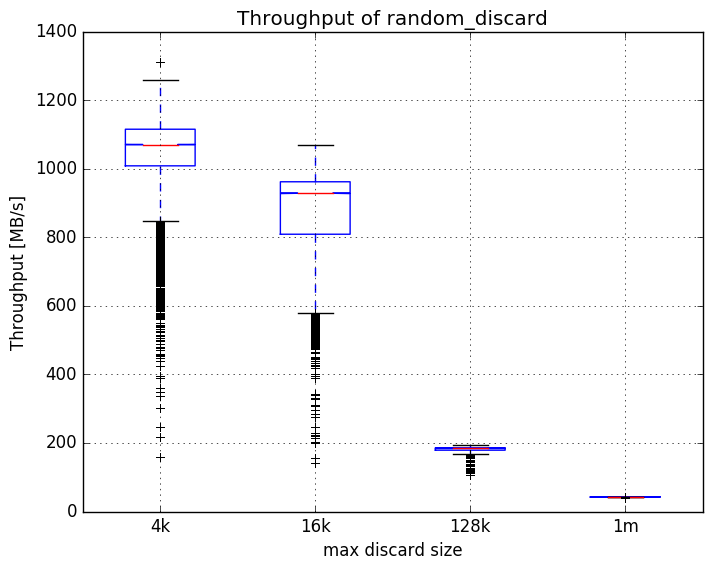
\includegraphics[width=\textwidth]{../results/discards/full_VDO/report/random_discard1_compare_boxplots}
\caption[Testing of VDO volume created with variable maximum discard size]{Testing of VDO volume created with variable maximum discard size. Prior to the test, the device was filled with random write workload}
\label{fig:discard-full}
        \centering
%        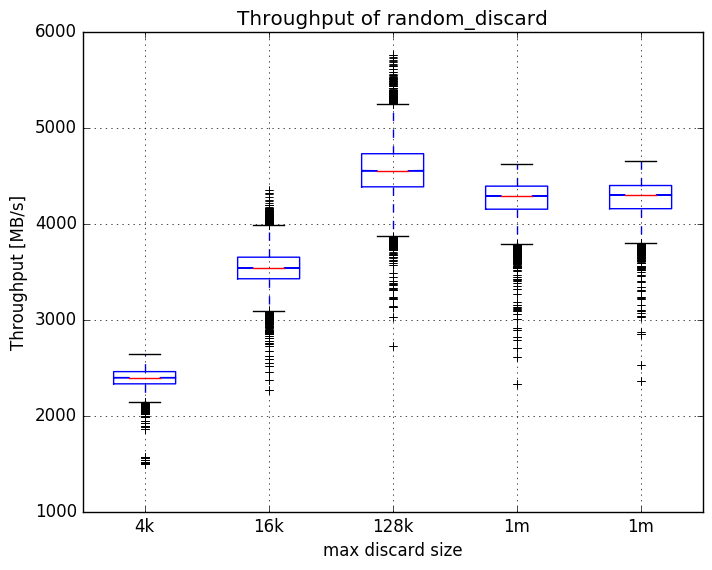
\includegraphics[width=\textwidth]{../results/discards/unalloc_VDO/report/random_discard1_compare_boxplots}
%\caption[Discards]{Testing of VDO volume created with various maxDiscardSize parameters. This test was conducted on a fresh unallocated instance of VDO}
%\label{fig:discard-unalloc}
        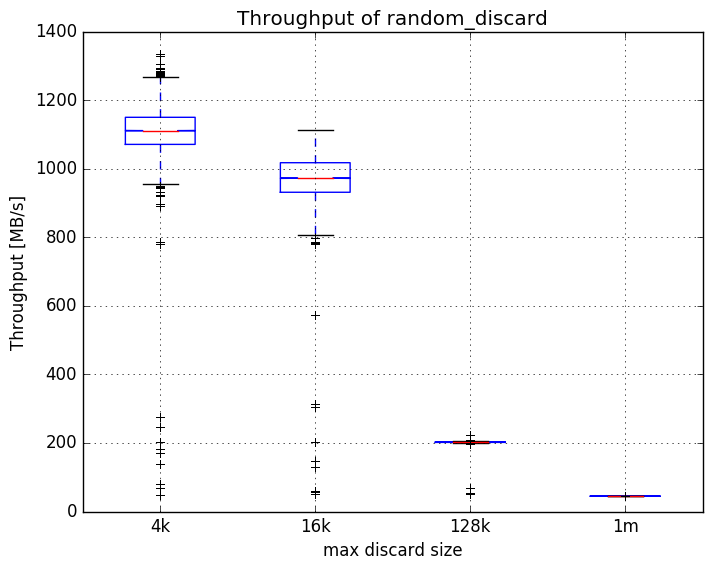
\includegraphics[width=\textwidth]{../results/discards/empty_VDO/report/random_discard1_compare_boxplots}
\caption[Testing of VDO volume created with variable maximum discard size on an empty VDO]{Testing of VDO volume created with variable maximum discard size on an empty VDO. The volume has been preallocated, but no additional data was written.}
\label{fig:discard-empty}
\end{figure}

\begin{table}
\centering
\begin{tabular}{|l|l|l|l|l|l|l|}
        \hline
        \multicolumn{7}{|l|}{Throughput of random discard (MB/s) on full VDO} \\ \hline
         & median & 1st q. & 3rd q. & min & max & stdev \\ \hline 
4k & 1077.65 & 1025.58 & 1119.79 & 158.12 & 1310.17 & 123 \\ \hline
16k & 935.4 & 863.6 & 966.42 & 140.93 & 1069.8 & 120 \\ \hline
128k & 184.27 & 179.58 & 185.94 & 105.26 & 195.25 & 9 \\ \hline
1m & 42.4 & 42.27 & 42.57 & 38.79 & 43.11 & 0 \\ \hline
\hline
        \multicolumn{7}{|l|}{Throughput of random discard (MB/s) on empty but fully allocatedVDO} \\ \hline
        & median & 1st q. & 3rd q. & min & max & stdev \\ \hline 
4k & 1114.18 & 1075.4 & 1152.95 & 48.4 & 1334.86 & 67 \\ \hline
16k & 977.27 & 935.99 & 1019.96 & 52.48 & 1111.36 & 62 \\ \hline
128k & 202.49 & 201.6 & 203.29 & 51.29 & 223.63 & 8 \\ \hline
1m & 44.87 & 44.75 & 45.03 & 44.31 & 46.67 & 0 \\ \hline
\end{tabular}
\caption{Table displaying performance od discard operation on a VDO volumes with various state of utilisation}
\end{table}

\clearpage

\section{Write policies}
VDO provides for different options for writing policies that are chosen with regard to the underlying device. 

In synchronised mode, VDO user assumes the data is written written to the persistent storage and no further commands are needed to make it persistent. User should set this option only when device under the VDO quarantees the data is written persistently when the write request is completed. If a volatile device is used with synchronous mode, user could potentialy lose data. This option should be used only when the used device has persistent write cache or a write-through cache.

In asynchronous mode, VDO does not guarantee the data is written to the persistent storage after the completion of write request. Only when the user or a structure using VDO issues flush command, it can be sure the data is written persistently.

Up until lately, VDO async mode was not compliant with ACID policy, which could result in unexpected data loss. ACID policy of asynchronous mode was introduced in RHEL-8.2, however, the old ACID non-compliant version was kept in VDO under the name async-unsafe for users that don't mind minor data loss and would see a performance problem using safe async.

It is important for developers to know the performance impact of writing policies, therefore performance testing should be conducted.

In this section, performance testing of the three available policies was conducted and the results can be observed on Figure~\ref{fig:writepolicies} and Table~\ref{tab:writepolicies}.

It is aparent that the synchronuous policy will be the slowest, since for every write request VDO have to flush data to a storage. However, more interesting observation can be made between ACID-compliant and unsafe asynchronous mode. Since VDO is an enterprised product, a lot of care needed to be taken so that the safe asynchronous mode will not slow down VDO considerably. We can see in the presented results that this effor was successfull.

\begin{figure}[!htb]
        \centering
        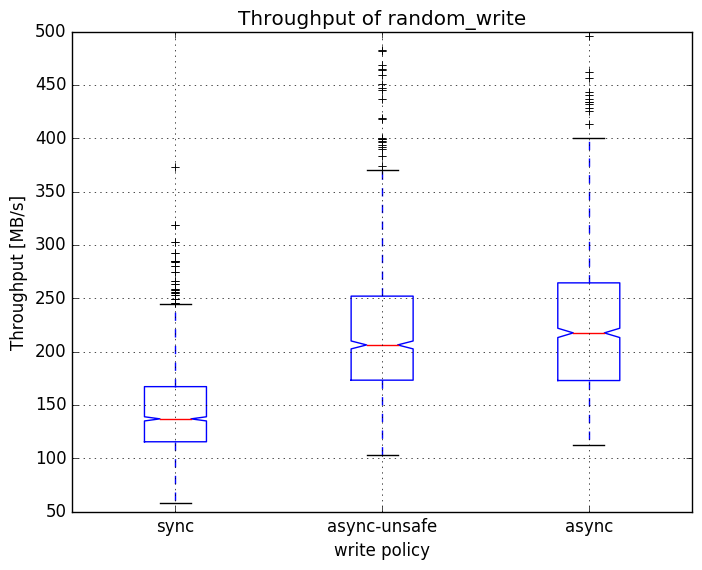
\includegraphics[width=\textwidth]{../results/write_policies/report/random_write1_compare_boxplots}
\caption[Performance of various write policies]{Testing of VDO volume created with various write policies. Synchronous, asynchronous and ACID non-compliant asnychronous-unsafe policy.}
\label{fig:writepolicies}
\end{figure}

\begin{table}
\begin{tabular}{|l|l|l|l|l|l|l|}
        \hline
        \multicolumn{7}{|l|}{Throughput of random write (MB/s)} \\ \hline
         & median & 1st q. & 3rd q. & min & max & stdev \\ \hline 
sync & 138.06 & 117.13 & 168.84 & 57.61 & 381.13 & 44 \\ \hline
async-unsafe & 212.87 & 177.17 & 258.17 & 99.24 & 510.32 & 66 \\ \hline
async & 207.14 & 172.57 & 253.68 & 92.76 & 539.94 & 69 \\ \hline
\end{tabular}
\caption[Performance of various write policies]{Testing of VDO volume created with various write policies. Synchronous, asynchronous and ACID non-compliant asnychronous-unsafe policy.}
\label{tab:writepolicies}
\end{table}

\section{Journal performance}
Recovery journal is an important aspect of VDO for assuring safety of user data. It is physically present in the last slabs of VDO storage, in the metadata part. Updating journal might not be an expensive operation, if the supporting device under VDO volume is fast enough. However, with increasing number of VDO users, use cases where VDO will be placed on a badly performing devices can emerge.

This experimend is aimed at exploring a use case where writing to a journal can be a bottleneck for the VDO performance.

The test was conducted using slow rotational hard drive on a Machine~\ref{hw:2}. Performance of this drive is very poor and installing VDO on top of it increases the performance. However, it would be interesting to observe if journaling is posing as a bottleneck and the VDO volume could be even faster.

VDO stores its metadata on the last slab (or multiple last slabs) of the physical device. By having the last slabs be actually on a completely different, fast device could show how much speeding the journal increases the overall performance of VDO.

We will start by creating a partition on the rotational drive. After putting this partition and the fast SSD into one volume group, we will create an LV on the partition and extendend it, so the last blocks are allocated from the second device. Finally, VDO can be put on top of this configuration and the test can be conducted.

Because the process of creating this configuration is not very intuitive, sequence of commands to do so is presented in~\ref{ex:fast-journal}

To make absolutely sure only the journal updates went to the fast device and not actual data, the test was run using seekwatcher, to examine block seeks. As can be seen on charts, data were kept strictly on the slow device part of the LV and only journal updates were handled by fast device.

One additional test was conducted by backing the journal with even more powerfull device. The ending region of VDO was spread over a part of NVMe SSD in hopes it would speed up the process even further. However, power of NVMe is in its number of queues. The process that handles VDO journaling is not multithreaded, as staded in Chapter 1. That is the reason why backing VDO with NVMe doesn't bring any additional benefits compared to a normal SSD.

We can observe the change in throughput using various hardware in a Figure~\ref{fig:journal-all}

\lstset{language=bash, 
numbers=none, 
frame=single, 
commentstyle=\color{blue}, 
basicstyle={\scriptsize\ttfamily}, 
keywordstyle=\color{black}, 
identifierstyle=\color{black}, 
stringstyle=\color{red},
captionpos=t,
showstringspaces=false,
breaklines=true,
breakatwhitespace=false,
tabsize=3,
caption={sdad},
}


\begin{lstlisting}[language=bash, label={ex:fast-journal}, caption={Creating a volume with last reagion on NVMe device}][frame=single]
    $ # /dev/sda1 is an 8GB partition on HDD
    $ # /dev/nvme0n1 is a 5GB partiiton on NVMe, however, size doesn't matter since we're only using first 2GB
    $ vgcreate vg /dev/sda1 /dev/nvme0n1
    $ lvcreate -n testLV1 -L 8g vg /dev/sda1
    $ lvextend vg/testLV1 -L 10g
    $ vdo create --name=testVDO --device=/dev/mapper/vg-testLV1  --vdoLogicalSize=80g
\end{lstlisting}

\begin{figure}[!htb]
        \centering
        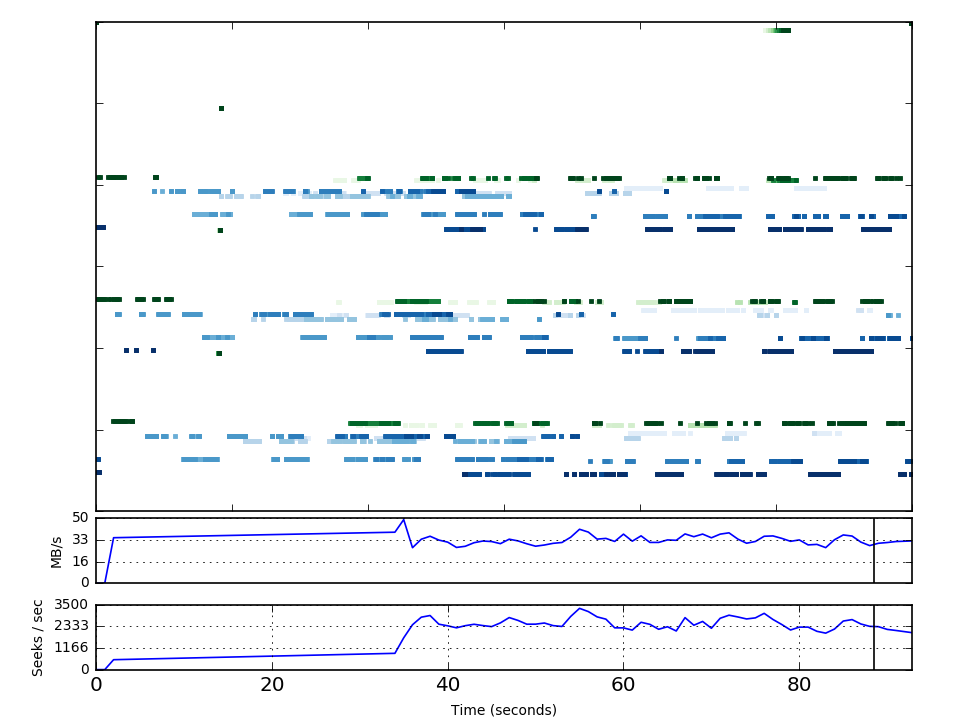
\includegraphics[width=\textwidth]{../results/journal/seeks/snaps/ssd_testlv}
\caption[Access pattern of VDO to data blocks on an underlying device]{Access pattern of VDO to data blocks on an underlying device.}
\label{fig:journal-LV}
        \centering
        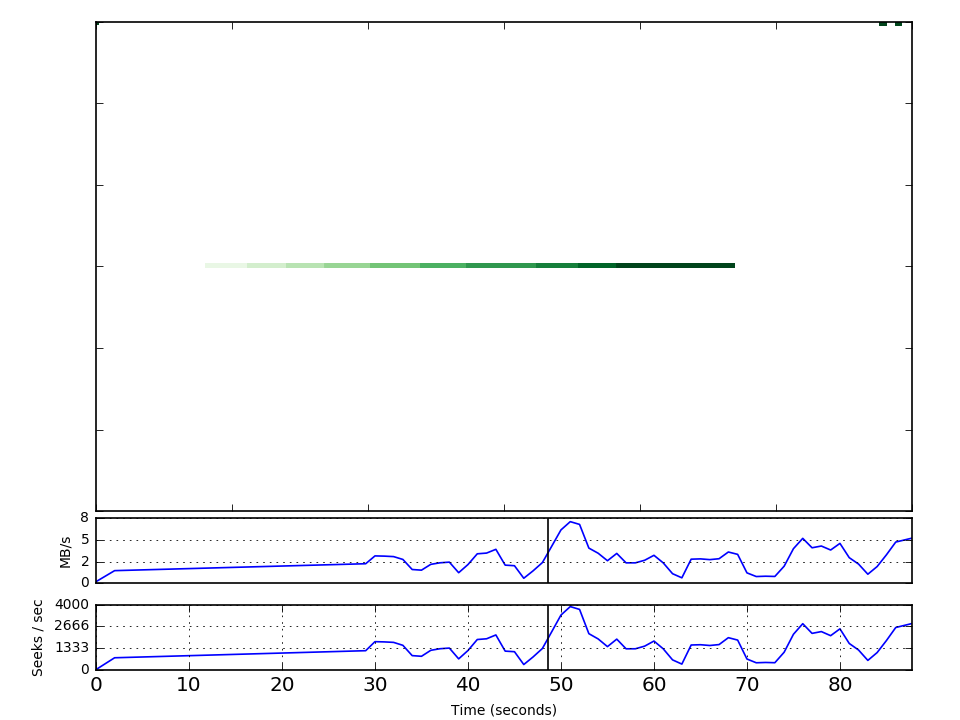
\includegraphics[width=\textwidth]{../results/journal/seeks/snaps/ssd}
\caption[Access pattern of VDO to the recovery journal.]{Access pattern of VDO to the recovery journal placed on additional fast storage.}
\label{fig:journal-SSD}
\end{figure}

\begin{figure}[!htb]
        \centering
        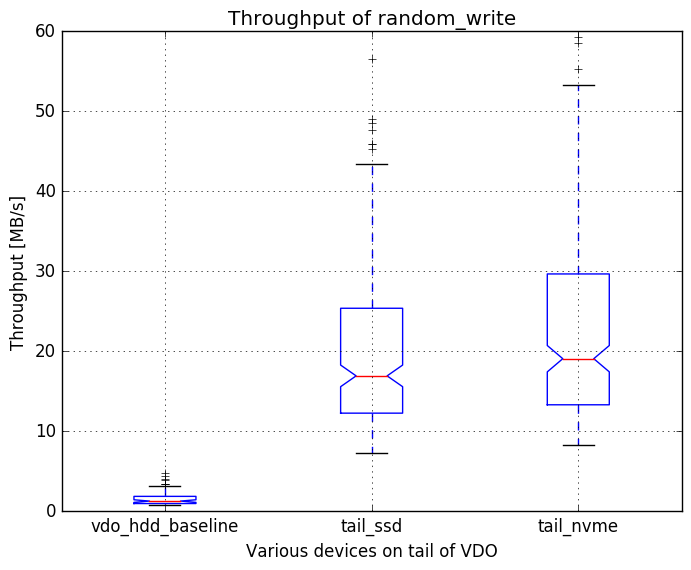
\includegraphics[width=\textwidth]{../results/journal/report/random_write1_compare_boxplots}
\caption[Performance of VDO with ending regions placed on different devices.]{Performance of VDO with ending regions placed on different devices. In the first test, the recovery journal is together with data blocks on an HDD. In the second and third test, the journal is forced on SSD and NVMe device respectively.}
\label{fig:journal-all}
\end{figure}

\begin{table}[!htb]
\centering
\begin{tabular}{|l|l|l|l|l|l|l|}
        \hline
        \multicolumn{7}{|l|}{Throughput of random write (MB/s)} \\ \hline
        test name & median & 1st q. & 3rd q. & min & max & stdev \\ \hline 
vdo\_hdd\_baseline & 1.28 & 0.97 & 1.87 & 0.85 & 4.73 & 0 \\ \hline
tail\_ssd & 16.93 & 12.27 & 25.38 & 7.29 & 152.26 & 28 \\ \hline
tail\_nvme & 19.08 & 13.32 & 29.67 & 8.27 & 149.68 & 21 \\ \hline
\end{tabular}
\caption[Performance of VDO with the ending regions placed on different devices.]{Performance of VDO with ending regions placed on different devices. In the first test, the recovery journal is together with data blocks on an HDD. In the second and third test, the journal is forced on SSD and NVMe device respectively.}
\label{tab:journal}
\end{table}
%\section{Aging testing}
%Aging test is a type of test that simulates usage for prolonged time. Resulting device layout is usually fragmented and its performance may be decreased. The volume can also spend considerable amout of time in near-full conditions. 

%To test this scenario, we will use multithreaded random write workload with occasional discard. VDO manual recommends to perform occasional large discard of unused blocks to save space and overhead. The test will be conducted on an NVMe device, since its cost may likely cause users to think about installing space saving software.



\chapter{Conclusion}
\label{conclusion}
The purpose of this thesis was to lay foundation of performance testing of Virutal Data Optimiser driver. This goal was achieved by explaining both principles of VDO space saving and VDO internal structures, then by explaining tuning mechanisms and providing workflow for performance testing as well as displaying many test results with reccomendations for correct VDO usage.

The purpose of VDO driver was explained along with mechanisms of space saving and data reduction. Following the basic principles, system requierements and VDO internal structures were introduced with emphasis on their impact on performance.

For the purposes of this thesis and future performance testing of VDO, many new features were implemented to a benchmark fs-drift, so that it can be used in a professional environment in order to test VDO and other block level layers thoroughly. These features significantly improve usability and possibilities of testing with fs-drift.

Along with implementation of features to fs-drift, a testing package compliant with Red Hat Kernel Performance automised workflow was created to execute tests and gather results. The results from these tests were processed by data processing library developed for this purpose.

In the testing part of this thesis, principles of VDO testing and tuning were explained and examined in practice. Each set of tests illustrates and clarifies the boundaries of VDO and shows different ways of performance testing of various VDO's components or a means to achieve a better performance. 

Results from the tests were processed into easily readable reports available in the electronic appendix. Subset of all generated graphs and tables was included in the main text in order to illustrate some of the main points.

Moreover, some of the tests designed for this thesis will be used for automised CI and Compose testing workflow in Red Hat Kernel Performance team. By conducting regular tests in a stable testing environment, performance of VDO can be under high quality supervision and possible issues can be found and removed effectively.












%\chapter{Tested configurations}
%\label{storageConf}
%In testing of specific storage stack layer, it is important to have performance assesment of a stack without that layer installed. These configurations are called baseline configurations. In this thesis, baseline configurations will used striped LVM to join hard drives as well as LVM cache to simulate real-life usage.

%After the baseline testing is finished, tests with VDO layer installed will be run. For non-cached version, only simple VDO layer will be installed with file system on top of it. In the cached version, VDO layer will be installed under the LVM-cache.


%\section{Baseline configurations}
%Baseline configurations will be storage stacks without the VDO layer installed. Their purpose is to provide a stable testing enviroment to determine performance of undelying hardware and performance of other layers in storage stack.

%\subsection{Striped LV}
%This baseline configuration will consist of simple stack built with LVM on top of two rotational hard drives. The striping of 2 will be used to balance the load on both devices equally. The commands %to create this simple stack is shown in example~\ref{ex:simpleLV}

%\lstset{language=bash, 
%numbers=none, 
%frame=single, 
%commentstyle=\color{dkgreen}, 
%basicstyle={\scriptsize\ttfamily}, 
%keywordstyle=\color{blue}, 
%identifierstyle=\color{blue}, 
%stringstyle=\color{red},
%captionpos=t,
%showstringspaces=false,
%breaklines=true,
%breakatwhitespace=false,
%tabsize=3,
%caption={sdad},
%}


%\begin{lstlisting}[language=bash, label={ex:simpleLV}, caption={Creating striped logical volume}][frame=single]
%    $ pvcreate /dev/sd[bc] -y
%    $ vgcreate vg /dev/sd[bc] -y
%    $ lvcreate -n testLV -i2 -l100%vg vg /dev/sd[bc] -y
%    $ mkfs.xfs /dev/mapper/vg-testLV        
%\end{lstlisting}

%\subsection{Cached LV}
%This baseline configuration will consist of a striped LV over two rotational hard drives supported with an LVM Cache hosted on a separate solid state device. These devices must belong to the same Volume Group. Creating LVM Cache consist of several steps. First a small part of the SSD needs to be reserved for LVM Cache metadata. This can be done by creating small LV on the device and converting that LV to cache-pool type. Next, we need to mark the portion of SSD we want to use for caching by creating another LV. We'll create another LV to join the two hard drives with striping of 2. At the end, we convert the storage LV to a cached volume. The commands to create this cached volume is shown in example~\ref{ex:cachedLV}

%\begin{lstlisting}[language=bash, label={ex:cachedLV}, caption={Creating cached logical volume}][frame=single]
 %   $ pvcreate /dev/sd[bce] -y
  %  $ vgcreate vg /dev/sd[bce] -y
   % $ lvcreate -n cacheMeta -L 44M vg /dev/sde -y
    %$ lvcreate -n cache -L 200G vg /dev/sde -y
%    $ lvcreate -n testLV -i2 -l100%vg vg /dev/sd[bc]  -y
 %   $ lvconvert --type cache-pool --poolmetadata vg/cacheMeta vg/cache -y
  %  $ lvconvert --type cache --cachepool vg/cache vg/testLV -y
    %$ mkfs.xfs /dev/mapper/vg-testLV        
%\end{lstlisting}


%\section{Configurations with VDO}
%After determining the performance without VDO layer installed, we can continue with actual performance testing of VDO. Important thing to notice is that when creating a file system on top of VDO volume, the file system will attempt to discard the whole volume to ensure a clean begining state. While testing this isn't really an important feature and with volumes of tens of tera bytes, it would take quite a long time to discard the whole VDO volume. Therefore mkfs options (-K for XFS) can be used to prevent it.

%\subsection{VDO over striped LV}
%This simple configuration will consist of VDO layer on top of two rotational hard drives joined by LV. The striping of 2 will be used to balance the load on both devices equally. The commands to create this stack is shown in example~\ref{ex:VDOLVC}

%\begin{lstlisting}[language=bash, label={ex:VDOLV}, caption={Creating VDO over striped LV}][frame=single]
%    $ pvcreate /dev/sd[bc] -y
 %   $ vgcreate vg /dev/sd[bc] -y
   % $ lvcreate -n testLV -i2 -l100%vg vg /dev/sd[bc] -y
  %  $ vdo create --name=testVDO --device=/dev/mapper/vg-testLV --vdoLogicalSize=60T  --vdoSlabSize=8g --force
    %$ mkfs.xfs -K /dev/mapper/vg-testLV      
%\end{lstlisting}

%\subsection{VDO under LVM Cache}
%This configuration will consist of a VDO layer built on top of two rotational hard drives joined by LV. The striping of 2 will be used to balance the load on both devices equally. Sometimes the LVM can have a problem with adding devices with different block size to a single volume group. This can be avoided by allowign mixed block sizes in lvm configuration file. Also, when more complexity needs to be build above the VDO layer, it is important to create a physical volume on a VDO block device. The commands to create this stack is shown in example~\ref{ex:VDOLVCache}

%\begin{lstlisting}[language=bash, label={ex:VDOLVCache}, caption={Creating cached VDO volume}][frame=single]
%    $ pvcreate /dev/sd[bce] -y
%    $ vgcreate vg /dev/sd[bc] -y
%    $ lvcreate -n testLV -i2 -l100%vg vg /dev/sd[bc]  -y    
 %   $ vdo create --name=testVDO --device=/dev/mapper/vg-testLV --vdoLogicalSize=60T --vdoSlabSize=8g --force    
  %  $ sed -i '/devices {/a allow_mixed_block_sizes = 1' /etc/lvm/lvm.conf
   % $ pvcreate /dev/mapper/testVDO -y
   % $ vgcreate VG2 /dev/mapper/testVDO /dev/sde -y -ff
   % $ lvcreate -n cacheMeta -L 44M VG2 /dev/sde -y
%    $ lvcreate -n cache -L 200G VG2 /dev/sde
 %   $ lvcreate -n testLV2 -l100%vg VG2 /dev/mapper/testVDO
  %  $ lvconvert --type cache-pool --poolmetadata VG2/cacheMeta VG2/cache -y
   % $ lvconvert --type cache --cachepool VG2/cache VG2/testLV2 -y
    %$ mkfs.xfs -K /dev/mapper/VG2-testLV2
%\end{lstlisting}


%\chapter{Conducted tests}
%For thorough testing of VDO, several types of tests needs to be executed. First section will aim to show differences in performance between loading VDO with heavily compressible data and non-compressible data. Next section will try to show differences in performance of VDO layer when under single threaded load and heavy multithreaded load. These tests will be held on all storage configurations from Chapter~\ref{storageConf}.

%\section{Different compressibility}
%The VDO layer can be used in multiple ways, when users want to save physical space. However, the level of compressibility of user data can vary. The aim of this test is to determine, whether compressibility of user data have impact on VDO performance or to what extent.

%\section{Single vs. Multithread}
%Since VDO usage is meant for simple users as well as for complex cases, it is important to know the differences between single-user load and heavy multithreaded traffic.



\chapter{Appendix}
\section{Testing hardware}
\label{hardware}
Testing hardware was borrowed form Red Hat Kernel performance team laboratory. The machines are powerfull enough to testing high performing drivers and tools. All storage devices used are regularly checked for health and immediately replaced if faulty.


\subsection{Machine\,1}
\label{hw:1}
This machine is used for regular testing of VDO and other complex layers in Red Hat Kernel Performance team. It's equiped with 4 $\SI{10}{\tera\byte}$ SAS rotational drives and one $\SI{220}{\giga\byte}$ SATA SSD for tests that require LVM Cache. The system is always installed on an additional SSD. This machine is equiped with enough memory to handle large VDO volumes.


\begin{table}
\centering
\begin{tabular}{|l|l|}
\hline
   \multicolumn{2}{|l|}{Machine\,1} \\ \hline %draven
    Model & Supermicro X11SPL-F\\
    \hline
    Processor & Intel Xeon Silver 4110  \\
    \hline
    Clock speed & $\SI{2.10}{\giga\hertz}$ (8 cores) \\
    \hline
    Memory & $\SI{49152}{\mega\byte}$ \\
    \hline
\end{tabular}
\caption{Testing machine 1}
\end{table}


\begin{table}
\centering
\begin{tabular}{|l|l|}
\hline
   \multicolumn{2}{|l|}{Testing Hard Drives (4x)} \\ \hline %draven
    Model & WD HGST Ultrastar\\
    \hline
    Capacity & $\SI{1}{\tera\byte}$  \\
    \hline
    Interface & SAS $\SI{12}{\giga\byte}$  \\
    \hline
    Type & Rotational HDD \\
    \hline    
    Logical sector size & $\SI{4096}{\byte}$ \\    
    \hline    
    Physical sector size & $\SI{4096}{\byte}$ \\
    \hline
    \hline
    \multicolumn{2}{|l|}{Testing SSD } \\ \hline %draven
     Model & Micron 5100 MTFD \\
    \hline
     Capacity & $\SI{240}{\giga\byte}$  \\
    \hline
    Interface & SATA $\SI{6}{\giga\byte}$  \\
    \hline
    Type & SSD \\
    \hline    
    Logical sector size & $\SI{512}{\byte}$ \\    
    \hline    
     Physical sector size & $\SI{4096}{\byte}$ \\
    \hline
    \hline
    \multicolumn{2}{|l|}{System disk} \\ \hline %draven
    Model & SuperMicro SSD  \\
    \hline
    Capacity & $\SI{126}{\giga\byte}$  \\
    \hline
    Interface & PCIe Gen3 x4 Lanes  \\
    \hline
    Type & SSD \\
    \hline    
   Logical sector size & $\SI{512}{\byte}$ \\    
    \hline    
    Physical sector size & $\SI{512}{\byte}$ \\
    \hline   
\end{tabular}
\caption{Testing devices instelled on Machine\,1}
\end{table}


\subsection{Machine\,2}
\label{hw:2}
This machine is used for regular testing of various file systems and storage layers. It's equiped with 3 $\SI{220}{\giga\byte}$ SATA SSD, one $\SI{220}{\giga\byte}$ SAS rotational HDD. Additionaly, there is one NVMe device.


\begin{table}
\centering
\begin{tabular}{|l|l|}
\hline
   \multicolumn{2}{|l|}{Machine\,1} \\ \hline %draven
    Model & Supermicro X11SPL-F\\
    \hline
    Processor & Intel Xeon Silver 4110  \\
    \hline
    Clock speed & $\SI{2.10}{\giga\hertz}$ (8 cores) \\
    \hline
    Memory & $\SI{49152}{\mega\byte}$ \\
    \hline
\end{tabular}
\caption{Testing machine 2}
\end{table}


\begin{table}
\centering
\begin{tabular}{|l|l|}
\hline
   \multicolumn{2}{|l|}{Testing Hard Drives} \\ \hline %draven
    Model & WD HGST Ultrastar\\
    \hline
    Capacity & $\SI{1}{\tera\byte}$  \\
    \hline
    Interface & SAS $\SI{12}{\giga\byte}$  \\
    \hline
    Type & Rotational HDD \\
    \hline    
    Logical sector size & $\SI{4096}{\byte}$ \\    
    \hline    
    Physical sector size & $\SI{4096}{\byte}$ \\
    \hline
    \hline
    \multicolumn{2}{|l|}{Testing SSDs 3x } \\ \hline %draven
     Model & Micron 5100 MTFD \\
    \hline
     Capacity & $\SI{240}{\giga\byte}$  \\
    \hline
    Interface & SATA $\SI{6}{\giga\byte}$  \\
    \hline
    Type & SSD \\
    \hline    
    Logical sector size & $\SI{512}{\byte}$ \\    
    \hline    
     Physical sector size & $\SI{4096}{\byte}$ \\
    \hline

    \hline
    \multicolumn{2}{|l|}{Tesing NVMe} \\ \hline %draven
     Model & Micron 5100 MTFD \\
    \hline
     Capacity & $\SI{240}{\giga\byte}$  \\
    \hline
    Interface & SATA $\SI{6}{\giga\byte}$  \\
    \hline
    Type & SSD \\
    \hline    
    Logical sector size & $\SI{512}{\byte}$ \\    
    \hline    
     Physical sector size & $\SI{4096}{\byte}$ \\

    \hline
    \multicolumn{2}{|l|}{System disk} \\ \hline %draven
    Model & SuperMicro SSD  \\
    \hline
    Capacity & $\SI{126}{\giga\byte}$  \\
    \hline
    Interface & PCIe Gen3 x4 Lanes  \\
    \hline
    Type & SSD \\
    \hline    
   Logical sector size & $\SI{512}{\byte}$ \\    
    \hline    
    Physical sector size & $\SI{512}{\byte}$ \\
    \hline   
\end{tabular}
\caption{Testing devices instelled on Machine\,2}
\end{table}

\clearpage
\section{Additional results}
During writing this thesis, many tests were conductend with various state of VDO and benchmark configurations thant could not have been all presented in the main text. However, some of the statements are referncing these results, so they could be viewed here.

\subsection{Discard performance of unallocated VDO}
In the Chapter~\ref{testing}, peculiar behavior discard operation of unallocated blocks in VDO was mentioned. Since VDO recognise that the discard requests are aimed on unallocated blocks, it doesn't do any work and only returns ackknowledgement. That is the reason why discard size doesn't affect VDO discard performance on unallocated storage.

\begin{figure}
\centering
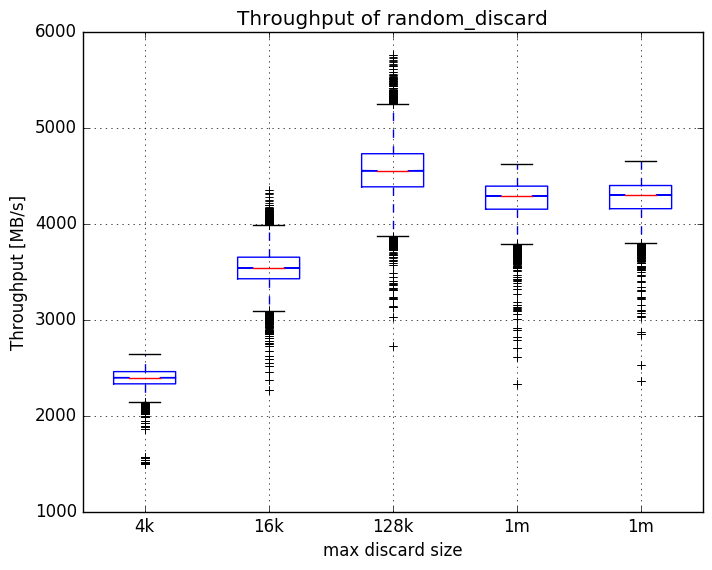
\includegraphics[width=\textwidth]{../results/discards/unalloc_VDO/report/random_discard1_compare_boxplots}
\caption[Performance of discard operation on an unnallocated VDO volume.]{This test was conducted on a fresh, unallocated instance of VDO volume. The performance appears to be high because of attempts are being made to discard blocks that are not in the mapping tree.}
\label{fig:discard-unalloc}
\end{figure}






\printbibliography[heading=bibintoc]


















\end{document}
